% !Mode:: "Tex:UTF-8"
\chapter{路由路径压缩与恢复机制}
\label{chap:5}
第三、四章研究了不依赖位置关系的拓扑骨干提取和虫洞拓扑识别问题,本章研究拓扑压缩的另一项重要研究内容,即路由路径的压缩和恢复技术。在大规模无线传感器网络中,为了提供可靠的数据传输和细粒度的系统管理,追踪数据包的路由路径非常重要。实时的路径记录功能使网络用户能够以细粒度的方式观察数据的传输和分析网络的状态。但由于无线传感器网络中严格的资源限制,要在每个数据包中记录完整的路径信息是非常困难的。很多的研究工作都尝试利用数据包路由路径信息,但都没能做到记录每个数据包的完整路径信息。本章致力于在每个数据包引入较低的常数开销的情况下记录完整和精确的路径路径,提出了基于哈希的路径压缩和恢复机制,命名为PathZip。PathZip的基本思想是将开销从传感器节点转移至能力较强的汇聚节点或基站。在数据包的传输过程中,经过的每个节点执行一次简单的哈希计算,将哈希值作为路径的标识储存在数据包中。汇聚节点获得路径标识后,通过重新计算哈希值重构出完整的路径。另外,PathZip利用了分别基于拓扑和基于几何的技术,通过开发路由路径之间的拓扑和几何相关性来降低算法的开销。本章通过理论分析和大量的仿真实验验证了PathZip方法的有效性和性能。
\section{引言}
数据收集是无线传感器网络中最基本和重要的功能,因此提高数据收集的可靠性一直是该领域中一个重要的研究热点。随着无线传感器网络的规模日益扩大,近年来出现了一系列大规模实际部署的系统,例如CitySee系统已经部署了超过2000个节点\upcite{CitySee}。日益增长的规模与其它一系列特性相结合,如动态的无线通讯链路、传感器节点的故障易发性,使得无线传感器网络系统的整体行为越来越复杂和难以预测\upcite{raj,post,miao}。系统状态可见性的缺失正日益成为大规模无线传感器网络实际部署所面临的重大挑战。

实时地追踪每个数据包的路由路径是一种以细粒度的方式观察网络行为和理解网络动态的重要手段。路径信息在之前的很多研究工作中得到了应用,如PAD\upcite{diagnosis_pad}设计了一种包标记算法来捕获数据包传输路径的变化,并利用这些信息对网络失效的原因进行分析。Sympathy\upcite{diagnosis_sympathy}是另一种网络诊断工具,通过动态地收集运行时的节点邻居表信息对网络的状态进行分析。利用数据包路由路径信息,就可以在基站对网络中很多问题进行分析,例如找出网络中负载较重的节点、检测路由环、检测路由路径的动态改变以判断潜在的节点失效、预测潜在的消息拥塞和网络健康状况等。

尽管利用数据包的路由路径信息可以给网络带来诸多的好处,但要实现以实时的方式记录每个数据包的完整和精确的路径信息是一项非常具有挑战性的任务。之前的很多研究工作虽然在这方面进行了一些尝试,但是都没能实现这一功能。例如,PAD仅在静态的网络中可以恢复出来自每个源节点的数据包的路由路径,当网络动态性较强(如路由路径频繁改变)的实际网络中,该方法的收敛时间变得较长甚至无法收敛。要实现这一目标,一种最原始和简单的想法是每个节点将自身ID存储在转发的每个数据包中,从源节点到汇聚节点的整个路径信息就能够被依次地记录在数据包中。但这种方式将导致数据包的大小显著增加,在数据包大小严格受限的无线传感器网络中并不可行,如802.15.4标准的MAC协议支持的数据包最大仅为127字节。另外,数据包大小的增加也将使数据传输的能量开销显著增加,因此无法应用在能量严格受限的无线传感器网络中。理想情况下,记录路径信息在数据包中占用的存储空间越小越好。因此,一种直观的改进方式就是对路由路径信息的数据进行压缩,将压缩后的路径信息存储在每个数据包中。但由于传统的无损压缩算法的输出随着输入数据量的增加而线性增长,这种方法仍将导致数据包大小随着路径长度的增加而线性增加。另外,路径信息的数据量极小(一般不超过200字节),在这种数据规模下,现有的压缩算法的压缩率较低。例如无线传感器网络中广泛使用的一种数据压缩算法LZW\upcite{compression_sensys}对结构化的传感器数据的压缩率一般不大于3。另外,由于压缩算法需要应用在每个数据包的逐跳的传输过程中,已有的压缩算法的计算开销对于资源、能力均严格受限的传感器节点来说也是难以接受的。综上所述,无线传感器网络的路由路径记录是一项亟需解决,且非常具有挑战性的研究内容,设计一种轻量级的路由路径记录机制已经成为实现大规模网络实际部署需要解决的关键技术问题。
\begin{figure}[t]
\centering
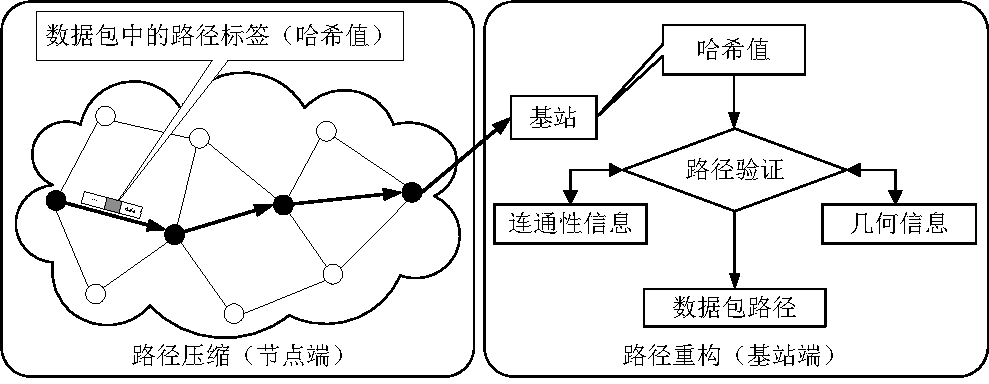
\includegraphics[width=0.8\textwidth]{fig501}
\caption{PathZip方法的原理和结构示意图}
\label{fig:501}
\end{figure}

本章提出了PathZip方法,在每个数据包中引入较低的固定开销的情况下,实时地追踪网络中每个数据包的路由路径。PathZip的基本思想是将计算开销从编码端(即传感器节点)转移至解码端(基站),并通过挖掘传感器节点和基站共有的先验知识(如网络拓扑、几何信息)来最小化需要从节点传输至基站的信息量。PathZip提供了一种灵活的框架,主要包括路径压缩和路径重构(或路径恢复)两个组件,如图\ref{fig:501}所示。路径压缩由作为编码端的传感器节点完成,以一种实时和被动的方式对所转发的数据包进行标记。具体来讲,在数据包传输过程中,经过的每个节点调用一个定制的哈希函数执行一次简单的哈希计算。哈希函数以当前节点的ID及数据包中记录的来自前一个节点的哈希值作为输入,通过计算得到一个新的哈希值。该哈希值作为路由路径的标识被记录在数据包中。基站作为解码端,利用路径验证过程对路由路径进行重构,通过遍历连接源节点和基站的所有可能的路径,重新计算出匹配的哈希值来确定初始的路由路径。网络拓扑信息作为一种有效的约束,被利用来降低路径验证过程的开销。另外,作为对PathZip的增强,本章还提出了几何辅助的路径重构机制,称为PathZip-G。PathZip-G利用几何信息(即节点位置)来进一步地降低路径重构过程的计算复杂度。具体来讲,PathZip-G设计了一种虚拟路径机制,使用较低的存储开销来记录数据包通过的近似几何区域。借此,路径验证过程的输入空间受到近似几何区域的约束,计算复杂度显著地降低。

就本文所知,本章是首次正式地提出并系统地研究无线传感器网络的路由路径记录问题。PathZip建立了一种解决路由路径记录问题的灵活的框架,设计了一种轻量级的定制的哈希函数,称为SPH(sensor path hash)。SPH致力于最小化每个数据包的传输和计算开销,其输出长度仅为8字节,计算复杂度是常用的哈希函数MD5的1/8。网络拓扑信息被充分地挖掘来降低基站在路径重构过程中的计算复杂度。本章还设计了基于分段线性近似(piece-wise linear approximation,PLA)的虚拟路径机算法PLA-VP,利用节点位置信息来进一步降低路径重构过程的计算复杂度。本章通过理论分析和大量的仿真实验验证了PathZip的有效性和性能,结果显示PathZip能够有效地记录无线传感器网络中每个数据包的精确路由路径,同时又保证了额外的计算和存储开销均比较合理。

本章余下的部分组织如下:5.2节阐述路由路径记录问题以及该问题的主要挑战;5.3节介绍PathZip路径压缩和恢复方法的具体设计;5.4节介绍几何辅助的路径重构机制PathZip-G;5.5节通过大量的仿真实验对方法的有效性和性能进行验证;最后5.6节对本章进行总结。
\section{问题描述}
本节对路由路径记录问题进行具体的描述,首先给出路径记录问题的定义,然后分析该问题的主要需求及其研究所面临的关键技术挑战。
\subsection{路由路径记录问题}
首先给出本章研究所采用的网络假设以及路径压缩问题的具体描述。本章考虑部署在平面区域上的无线传感器网络,假设网络中每个节点具有唯一的ID。网络通讯的连通关系图建模为一个简单无向图$G(V,E)$,其中点集$V$表示传感器节点,边集$E$表示节点之间直接的通讯链路。$P_{u,v}$表示节点$u,v$之间的一条路由路径。$X$表示网络中一个数据包,$P(X)$表示$X$的传输路径,$X$称为路径$P(X)$的拥有者(owner)。假设基站具有较强的计算和存储能力。网络在经过一段初始化过程后,就能够具有实时的路径记录功能,即能够获得网络中每个数据包的完整和精确的传输路径。定义\ref{def:501}给出了路由路径记录问题的具体定义。
\begin{definition}\label{def:501}
假设$X$表示网络$G$的初始化过程结束后,到达基站的任意一个数据包,$\mathcal{K}$表示基站收到数据包$X$后得到的有效信息。路由路径记录问题即提供一种机制$\mathcal{T}$,使得基站能够利用有限的信息$\mathcal{K}$,恢复出数据包$X$的完整的传输路径$P(X)$,即$\mathcal{T}(\mathcal{K})\to{P(X)}$。
\end{definition}
\subsection{需求和挑战}
基于无线传感网络的特性,路由路径记录问题的解决方案主要面临以下两个方面的需求和挑战。
\subsubsection{压缩率}
路由路径记录问题要求基站能够获得网络中每个数据包的完整传输路径。解决方案必须能够有效地对路径信息进行压缩,降低需要传输的数据量,同时还要求能够重构出精确的初始路径。因此,所采用的路径压缩机制必须能够提供良好的压缩率,并且压缩过程必须是无损的和可恢复的。

数据包的传输路径信息是在传输过程中动态地产生的,且来自每个源节点的数据包的传输路径经常随时间动态改变。因此为了使基站能够获得每个数据包的传输路径,必须将路径信息实时地记录在数据包本身中。由于无线传感器网络中数据包的大小严格受限,我们要求每个数据包中用来记录路径信息的存储空间是固定的,而与具体的路径长度无关。这一严格要求使得传统的数据压缩算法在路径记录问题中不可用,因为这些算法输出的数据量往往随着输入数据的增加而线性增长。实现固定输出的无损压缩是一个非常具有挑战性的问题,也正是本章所要研究的内容。
\subsubsection{计算和存储开销}
在路由路径记录问题中,路径信息的压缩算法将在每个数据包的逐跳传输中被频繁地调用。因此所采用的压缩算法必须是计算非常简单的,且存储开销极低的,才能够实际应用在资源严格受限的传感器网络中。传统的数据压缩算法无法满足路由路径压缩算法的要求。

基于以上需求,本章提出了一种轻量级的基于哈希的路由路径压缩和恢复方法PathZip,接下来将对该方法的基本原理和具体设计进行介绍。
\section{PathZip:基于哈希的路径压缩和恢复方法}
本节介绍PathZip路径压缩和恢复方法的具体设计,包括基于哈希的路径压缩和恢复机制,以及应用基于拓扑的技术来开发路由路径之间的拓扑相关性并降低路径恢复过程的开销。
\subsection{PathZip方法概述}
给定节点数量为$N$的网络$G$,在不采用压缩机制的情况下,完整地记录一条$k$跳路径需要的存储开销为$k\log{N}$位。这一开销随着路径长度的增加而增加,且对于数据包大小严格受限的传感器网络来说是过高的。在实际部署的大规模传感器网络系统如CitySee系统\upcite{CitySee}中,很多路径的长度已经超过了20跳。因此,必须引入一定的压缩机制来降低数据包中的存储开销,最理想的情况是能够保持固定的开销。

首先,我们通过利用网络的拓扑信息来开发路由路径之间的拓扑相关性,从而降低路径信息的数据量。网络中的一条$k$跳路径,可以被看作是包含$k+1$个节点的序列。这$k+1$个节点之间并不是毫无关联的,而是受到网络通讯图的约束,节点之间存在一定的拓扑关联性。因此,本章提出一种简单且有效的机制,开发路由路径之间的拓扑相关性。具体来讲,每个节点为自己的直接邻居建立局部的ID,则索引任意的一个邻居仅需最多$\log\Delta$位,其中$\Delta$表示最大节点度。当一个节点转发数据包时,就可以通过局部ID来记录下一跳节点,而无需记录节点的全局ID。因此,完整地记录一条$k$跳路径,仅需最多$k{\log\Delta}$位存储开销,远低于使用全局ID需要的$k{\log{N}}$位。

然后,PathZip方法采用了一种基于哈希的技术,进一步将变化的存储开销转化为固定长度的压缩输出。哈希函数是一种确定性的过程,能够将一个任意长度的位串数据映射成一个固定长度的输出位串。另外,哈希函数的另外一个重要的优势是哈希值的计算过程非常简单。因此,本章巧妙地利用哈希函数的这些特性,将其应用在无线传感器网络的路由路径记录问题中,设计了基于哈希的路径压缩机制。下面介绍其基本原理和过程。源节点产生一个数据包后,调用哈希函数,以自身ID和一个预设的初始化串作为输入,计算得到一个哈希值,并将该哈希值保存在数据包中。随后,数据包每到达一个新的节点,调用同一个哈希函数,以自身ID和数据包中保存的上一跳节点计算得到的哈希值作为输入,计算得到一个新的哈希值。该哈希值作为一个动态变化的标签,实时地记录下数据包的路径信息,并随着数据包一起被发送至基站。至此,仍然有两个问题需要解决:第一,传统的通用哈希函数的计算尽管非常简单,但应用于无线传感器网络中每个数据包的逐跳传输中,其计算开销和存储开销仍然太高;第二,由于哈希函数的计算过程是不可逆的,要得到初始的路由路径,还需要设计一种机制从哈希值恢复出初始的路径信息。

为了解决第一个问题,本章设计了一种定制的轻量级的哈希函数SPH。SPH的输出长度为64位,而计算开销仅为常用的哈希函数MD5的1/8,从而有效地降低了路径压缩过程的计算和存储开销。本节后面的内容将对SPH的设计进行具体的介绍。

为了解决第二个问题,本章设计了基于哈希的路径恢复机制,其基本思想是利用哈希函数的抗冲突性。哈希函数的抗冲突性定义为:对于哈希函数$h=H(M), h:{\{0,1\}}^{*}\to{\{0,1\}}^n$,仅通过计算无法找出两个不同的输入$x^{'}\neq{x}$,使得$H(x^{'})=H(x)$,其中$n$是函数输出的长度。也就是说,对于任意两条不同的路径,通过哈希计算得到的哈希值相同的概率极低,而通过计算无法找出这样的两条路径。基于这一特性,每条路由路径都可以被映射成一个确定且独有的哈希值。反过来讲,每个哈希值对应于唯一的一条路由路径。因此,当每个数据包达到基站后,基站根据数据包的源节点和路径长度信息,找出所有可能的路由路径,分别计算这些路径的哈希值,并与数据包中保存的哈希值进行对比。这一过程称为路径的验证。一旦在路径验证过程中得到相同的哈希值,就能够恢复出该数据包的路由路径。另外,PathZip 方法充分利用网络拓扑信息,挖掘路由路径之间的相关性,从而减少路径验证过程中候选路径的数量,降低路径恢复的计算复杂度。

PathZip方法主要具有三个方面的优势。第一,PathZip将大部分的计算复杂度从传感器节点转移至基站,而每个数据包中额外的存储开销非常低,从而有效地降低节点的计算和通讯开销,节约了节点能量。第二,PathZip充分地利用了路由路径之间的拓扑相关性,降低了基站中路径恢复过程的计算复杂度。第三,PathZip还能够充分利用数据包之间的时间相关性。每个计算出的哈希值及其对应的路径信息都被储存在基站中。当新的数据包到达基站后,首先读取数据包中保存的哈希值,并与已储存的信息进行比对,如果找到了相同的哈希值就可以直接得到对应的路由路径。也就是说,对于网络中每条可能的路由路径,PathZip仅需执行一次路径验证过程。在相对稳定的网络中,来自每个源节点的数据包的路由路径也相对稳定。因此在网络经历了一段初始化过程后,往往能够仅通过查询历史信息就可以恢复出路由路径。
\begin{algorithm}[t]
\caption{SPH压缩算法}
\label{alg:501}
\begin{algorithmic}[1]
\REQUIRE ~~\
32位节点ID输入块$M$,64位的初始化向量$IV$
\ENSURE ~~\
64位哈希值$H$
\IF {当前节点是源节点}                                       \label{alg:501:01}
    \STATE 将$IV$切割成4个16位的块$A,B,C,D$;                \label{alg:501:02}
\ELSE                                                        \label{alg:501:03}
    \STATE 从数据包中读取上一跳节点的哈希值$H$;             \label{alg:501:04}
    \STATE 将$H$切割成4个16位的块$A,B,C,D$;                 \label{alg:501:05}
\ENDIF                                                       \label{alg:501:06}
\STATE 将$M$切割成两个16位的块$M[0],M[1]$;                  \label{alg:501:07}
\STATE $a:=A, b:=B, c:=C, d:=D$;                            \label{alg:501:08}
\FOR {$i=1$ to 8}                                            \label{alg:501:09}
    \IF {$1\leq{i}\leq{2}$}                                  \label{alg:501:10}
        \STATE $f:={(b\land{c})}\lor{(\neg{b}\land{d})}$;   \label{alg:501:11}
    \ELSIF {$3\leq{i}\leq{4}$}                               \label{alg:501:12}
        \STATE $f:={(b\land{d})}\lor{(c\land{\neg{d}})}$;   \label{alg:501:13}
    \ELSIF {$5\leq{i}\leq{6}$}                               \label{alg:501:14}
        \STATE $f:=b\oplus{c}\oplus{d}$;                    \label{alg:501:15}
    \ELSIF {$7\leq{i}\leq{8}$}                               \label{alg:501:16}
        \STATE $f:=c\oplus{(b\lor{\neg{d}})}$;              \label{alg:501:17}
    \ENDIF                                                   \label{alg:501:18}
    \STATE $temp:=d,d:=c,c:=b$;                             \label{alg:501:19}
    \STATE $b:=b+$leftrotate$(a+f+M[i\bmod2]+T[i],s[i])$;   \label{alg:501:20}
    \STATE $a:=temp$;                                       \label{alg:501:21}
\ENDFOR                                                      \label{alg:501:22}
\STATE $A:=A+a, B:=B+b, C:=C+c, D:=D+d$;                    \label{alg:501:23}
\STATE $H:=A\|B\|C\|D$;                                     \label{alg:501:24}
\end{algorithmic}
\end{algorithm}
\subsection{SPH哈希函数设计}
PathZip设计了一种轻量级、抗冲突的哈希函数SPH。首先以MD5为例分析为什么通用的哈希函数无法应用在路由路径记录问题中。MD5将一个任意长度的输入切割成一系列512位的块,经过计算得到一个128位的哈希值。虽然MD5已经被普遍认为是计算非常简单的,但仍无法直接应用于无线传感器网络的路由路径记录问题。原因主要包括三个方面:第一,PathZip以节点ID作为哈希函数的输入,若采用MD5则需要将节点ID转化成512位的输入块,这将引起不必要的存储和计算开销;第二,MD5是集中式计算方式,而PathZip需要一种分布式的方案,因为路由路径是随着数据包的传输实时地产生的;第三,路径压缩问题的输入空间相对于MD5无限大的输入空间是非常有限的,因此无需采用MD5中128位的较长输出。较短的输出足以提供充分的抗冲突性,同时又可以节约数据包的存储空间。基于以上分析,PathZip设计了SPH哈希函数,采用更短的输入和输出,且具有更低的计算复杂度。具体来讲,SPH采用32位输入(由每个节点的ID转换得到),并将任意长度的路径信息映射为64位的哈希值。

SPH的具体执行流程如算法\ref{alg:501}所示,主要分为两个过程:设计压缩函数,利用压缩函数构建哈希函数。压缩函数以两个长度分别为64位和32位的二进制串作为输入,其中64位串来自一个预设的初始化向量$IV$(或数据包中储存的上一跳节点计算的哈希值),32位串由当前节点的ID转换得到。SPH将64位输入串切割成4个16 位的块$A,B,C,D$(第\ref{alg:501:01}-\ref{alg:501:06}行),将32位输入块$M$切割成2个16位的块$M[0],M[1]$(第\ref{alg:501:07}行)。输入块的处理包括四轮,每轮包括两次相似的操作。每一轮调用一个不同的非线性函数$f$(第\ref{alg:501:10}-\ref{alg:501:18} 行),结合$M[0]$和$M[1]$进行计算(第\ref{alg:501:19}-\ref{alg:501:21}行)。最后,算法得到一个64位串作为哈希计算的结果(第\ref{alg:501:24}行)。因此,SPH对每次输入执行8次运算,而MD5需要执行64次计算。

接着,我们采用Merkle-Damgard结构\upcite{damgard},利用上述的压缩函数构造出SPH哈希函数,如图\ref{fig:502}所示。每个节点调用压缩函数,以当前节点的ID 和前一个节点的输出作为输入,计算得到新的值,并保存在数据包中。在数据包的传输过程中,该值被不断地更新,并随着数据包被发送至基站。在数据包的整个传输过程,迭代的计算过程就构成了SPH哈希函数,而最终的计算结果就代表了路径的哈希值。
\begin{figure}[h]
\centering
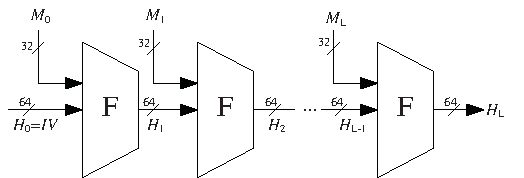
\includegraphics[width=0.75\textwidth]{fig502}
\caption{SPH采用的Merkle-Damgard结构}
\label{fig:502}
\end{figure}

下面分析SPH函数的抗冲突性。在随机预言机模型\upcite{bookcryp}下,压缩函数被视为理想的黑盒。通常的冲突攻击(如生日攻击)要实现找到一次冲突的概率大于1/2,需要的计算复杂度为$1.17\times2^{n/2}$,其中$n$为输出的长度。因此,SPH在理想情况下的抗冲突性能是$1.17\times2^{32}$。对于$Q$个不同的输入,出现冲突的结果的概率为:
\begin{equation}\label{equ:601}
\sigma=1-\left(\frac{2^{32}-1}{2^{32}}\right)\left(\frac{2^{32}-2}{2^{32}}\right)\ldots\left(\frac{2^{32}-Q+1}{2^{32}}\right)
\end{equation}

在本章后面的实验评估部分,我们还将对SPH哈希函数的抗冲突性进行具体的实验验证。
\subsection{计算复杂度分析}
下面分析PathZip路径压缩和恢复方法的计算复杂度。PathZip的计算开销主要包括两部分,分别对应于编码端的路径压缩过程和解码端的恢复恢复过程。在编码端,传感器节点调用SPH哈希函数实时地对路由路径进行压缩。SPH的计算复杂度前面已经进行了分析,下面主要分析解码端的路径恢复过程的开销。在解码端,基站利用较强的存储和计算能力,通过重新计算哈希值恢复出初始的路径。在不利用任何辅助信息的情况下,路径恢复过程的计算复杂度(即需要执行哈希计算的候选路径的条数)的上限为$P_N^{k-1}$,其中$N$表示整个网络中的节点数量,$k$表示路径的跳数。为了降低计算复杂度,PathZip利用网络拓扑信息来挖掘路由路径之间的拓扑相关性。假设每个节点知道自己的最大的邻居集合,基站知道每个节点的最大的邻居集合。在进行路经验证时,只需要考虑那些符合实际的网络连通性的可能的路径。再利用数据包中包含的源节点和路径长度信息,可以进一步地缩小候选路径的范围。那么,一条$k$跳路径的恢复过程的计算复杂度的上限降低为$\Delta(d-1)^{k-2}$,其中$\Delta$表示节点度的最大值。

通过利用拓扑信息对路由路径的约束,PathZip有效地降低了路径恢复过程的开销的理论上限值。而实际的计算开销比理论值要低得多,本章后面的实验部分还将进行具体的实验验证。另外,计算复杂度的上限仅提供一个理论的结果,而在实际的协议运行过程中,来自每个源节点的数据包的路由路径的数量还将受到具体的路由算法的限制。再结合历史信息的记录,每条可能的路由路径仅需要执行一次哈希值计算。在网络运行一段时间后,大部分可能的路径的哈希值都已经得到,系统就可以仅通过查询历史信息来恢复数据包的路由路径。
\section{PathZip-G:几何辅助的路径恢复机制}
本节介绍几何辅助的路径恢复机制,在网络几何信息(即节点位置)可用的情况下,通过挖掘节点之间的几何相关性(即空间相关性)来进一步降低路径恢复过程的开销。作为对PathZip方法的增强,几何辅助的路由恢复机制被称为PathZip-G。PathZip-G提出了一种虚拟路径机制,并设计了分段线性近似(PLA)的虚拟路径算法。下面首先介绍PathZip-G的基本思想,然后分别对虚拟路径机制和PLA虚拟路径算法进行具体地介绍。
\subsection{PathZip-G方法概述}
首先,PathZip-G假设网络中每个节点的位置信息是可知的,这可以通过利用大量的网络定位技术来实现\upcite{LLL}。下面介绍PathZip-G的基本思想和主要过程。

为了追踪数据包的路由路径,我们在数据包中记录下数据包经过的部分节点。这些节点是按照某种精心设计的原则被选择出来的,使得路径中其它所有的节点与这些选定节点之间具有一定的几何近似关系。具体来讲,其它的所有节点都会落在一个由选定节点确定的近似几何区域内。接下来,在基站中就可以利用节点的位置信息找出位于该近似几何区域内的所有节点,并且仅需要将这些节点作为候选节点来执行路径的验证过程。通过这种方式,候选节点的数量以及对应的候选路径的数量都将显著地减少,从而使得路径恢复过程的计算开销显著地降低。图\ref{fig:503}给出了路径的近似几何区域的一个简单示例。在图示的网络连通图中,一个数据包沿着路径$\{A,B,C,D,E\}$从节点$A$发送至节点$E$。在仅利用网络连通性信息的情况下,验证这条路径需要将除$A$和$E$之外的11个节点作为候选节点,由此产生的可能的4跳路径的数量为12。如果能够得到图中灰色矩形区域所示的近似几何区域,候选节点的数量将减少为5,由此产生的候选路径的数量相应地减少为4。
\begin{figure}[h]
\centering
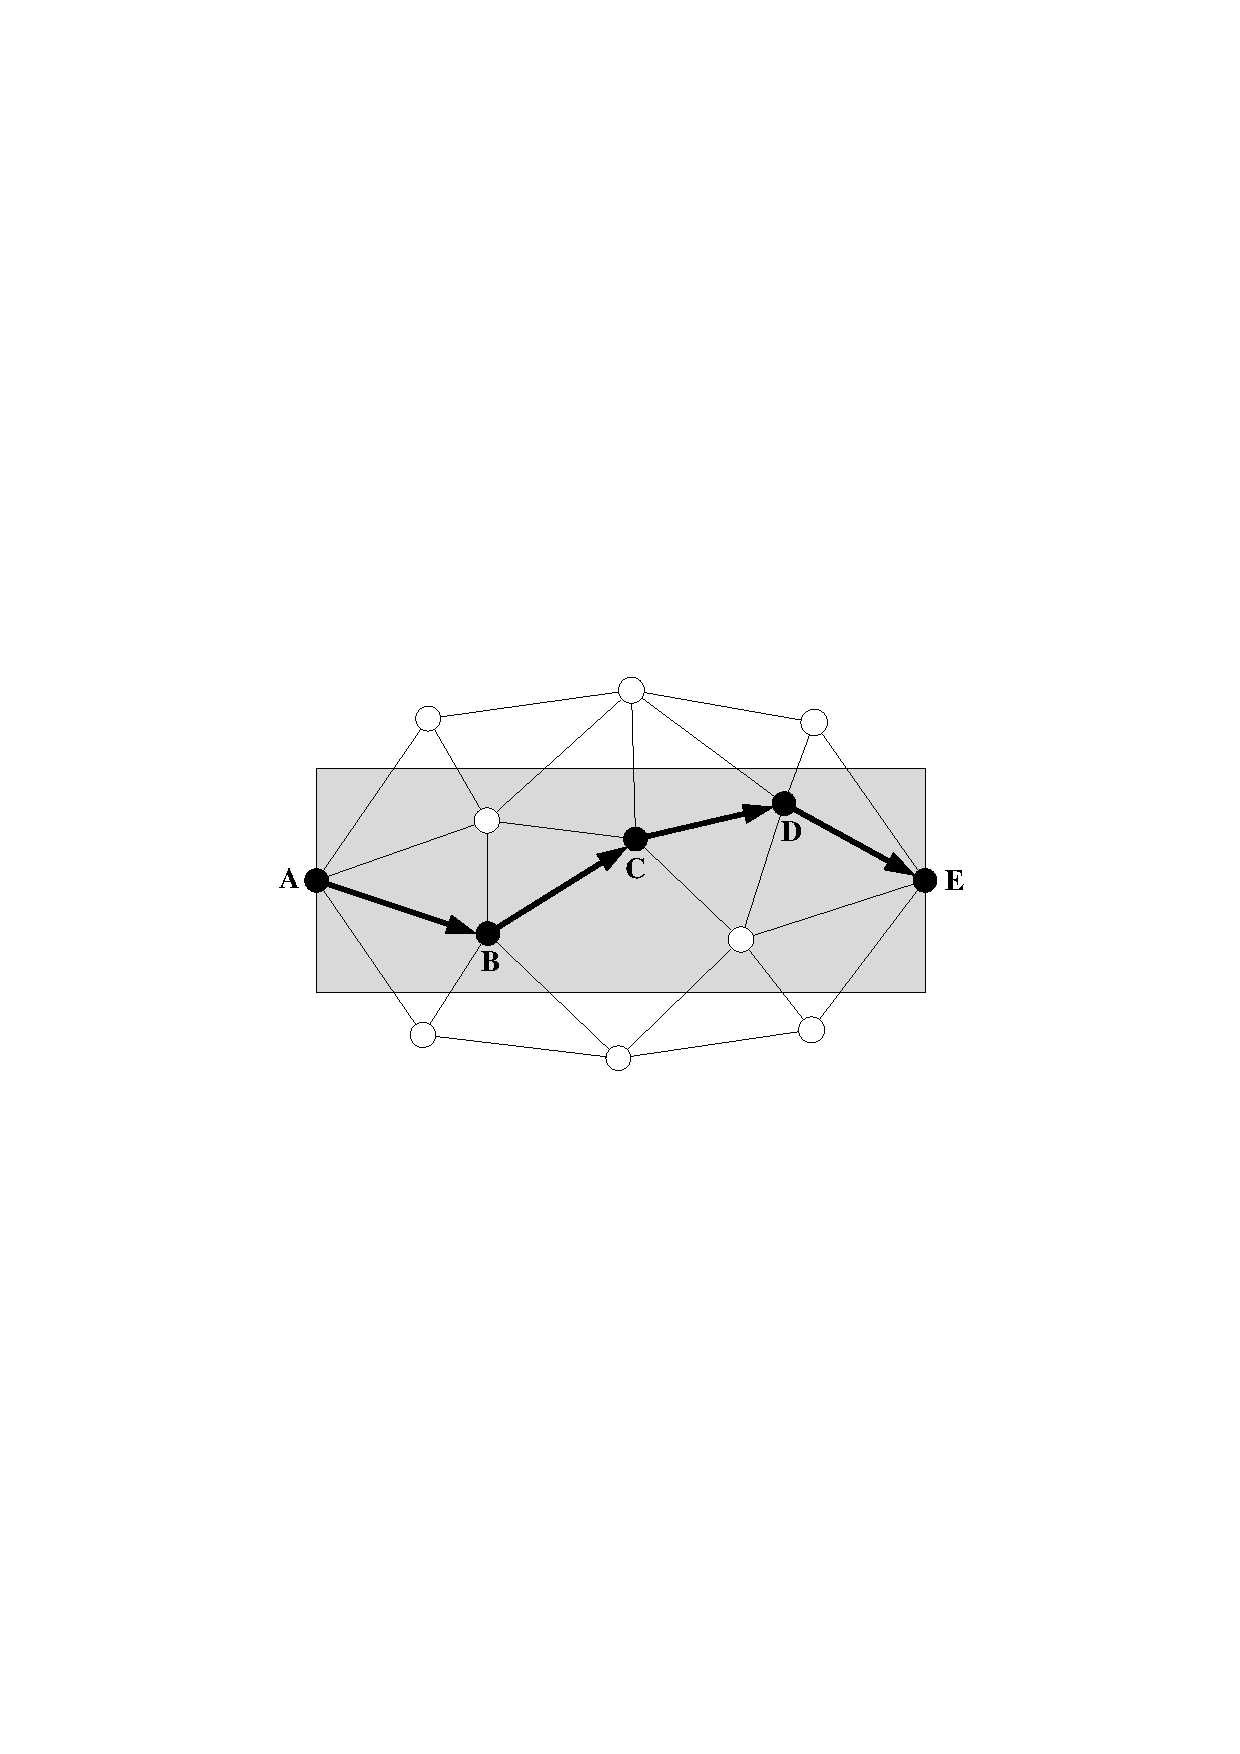
\includegraphics[width=0.45\textwidth]{fig503}
\caption{路由路径的近似几何区域的示例}
\label{fig:503}
\end{figure}

至此,PathZip-G还需要解决两个问题。第一,需要设计一种机制来记录路由路径的近似几何区域;第二,需要尽量地降低由记录路径的近似几何区域带来的额外计算和存储开销,尤其是传感器节点的开销。为了解决这两个问题,PathZip-G引入了基于PLA技术的虚拟路径机制。
\subsection{虚拟路径机制}
PLA问题在过去的几十年中得到深入地研究,并被广泛应用于很多领域中,如数字曲线描述\upcite{pla_curve}、时间序列近似\upcite{pla_timeseries},以及无线传感器网络的数据压缩\upcite{compression_tpds,pla_sensordata}等。PLA问题的基本思想是在保证有限误差$\varepsilon\geq0$的基础上,利用最小数量的近似线段或者点来近似地描述对象(如数字曲线、时间序列、数据流等)。

从几何的角度来看,一条路由路径可以被看作平面上的一条二维折线。因此可以利用PLA方法,用路径上的部分节点形成的线段来近似地描述整条路径,同时保证其它的所有节点与近似线段之间的距离不超过某一上限值$\varepsilon$。按照这种方式选择出来的节点就构成了原始路径的虚拟路径。也就是说,完整的路由路径一定位于由虚拟路径和$\varepsilon$确定的近似几何区域内。如图\ref{fig:504a}所示,带箭头的黑实线表示一条真实的6跳路径,而${\{n_1,n_5,n_7\}}$则构成了它的一条虚拟路径,其它的所有节点到虚拟路径的垂直距离不大于误差上限$\varepsilon$。定义\ref{def:502}给出了基于PLA的虚拟路径的形式化描述。
\begin{definition}\label{def:502}
给定一条路径$P$,误差测量函数$err()$,以及误差上限值$\varepsilon$,利用PLA算法找出点集$P^{'}$,使得$err(P,P^{'})\leq\varepsilon$,则$P^{'}$即为路径$P$的虚拟路径。当$P^{'}$中点的数量$|P^{'}|$达到最小化时,$P^{'}$为最优的虚拟路径。比值$|P|/|P^{'}|$为虚拟路径的压缩率。
\end{definition}
\subsection{PLA虚拟路径算法}
PathZip-G利用虚拟路径机制来简化路径恢复过程。但为了储存虚拟路径信息,PathZip-G必须在数据包中引入额外的存储开销。实现额外存储开销的最小化就成为虚拟路径算法设计的主要目标。因此,在进行基于PLA的虚拟路径算法设计时,要尽量减少虚拟路径中节点的数量。另外,由于路由路径是随着数据包的传输而实时和增量式地产生的,因此必须设计一种实时的在线算法。
\begin{figure}[t]
  \centering
  \subfloat[虚拟路径由真实节点构成]{
    \label{fig:504a}
    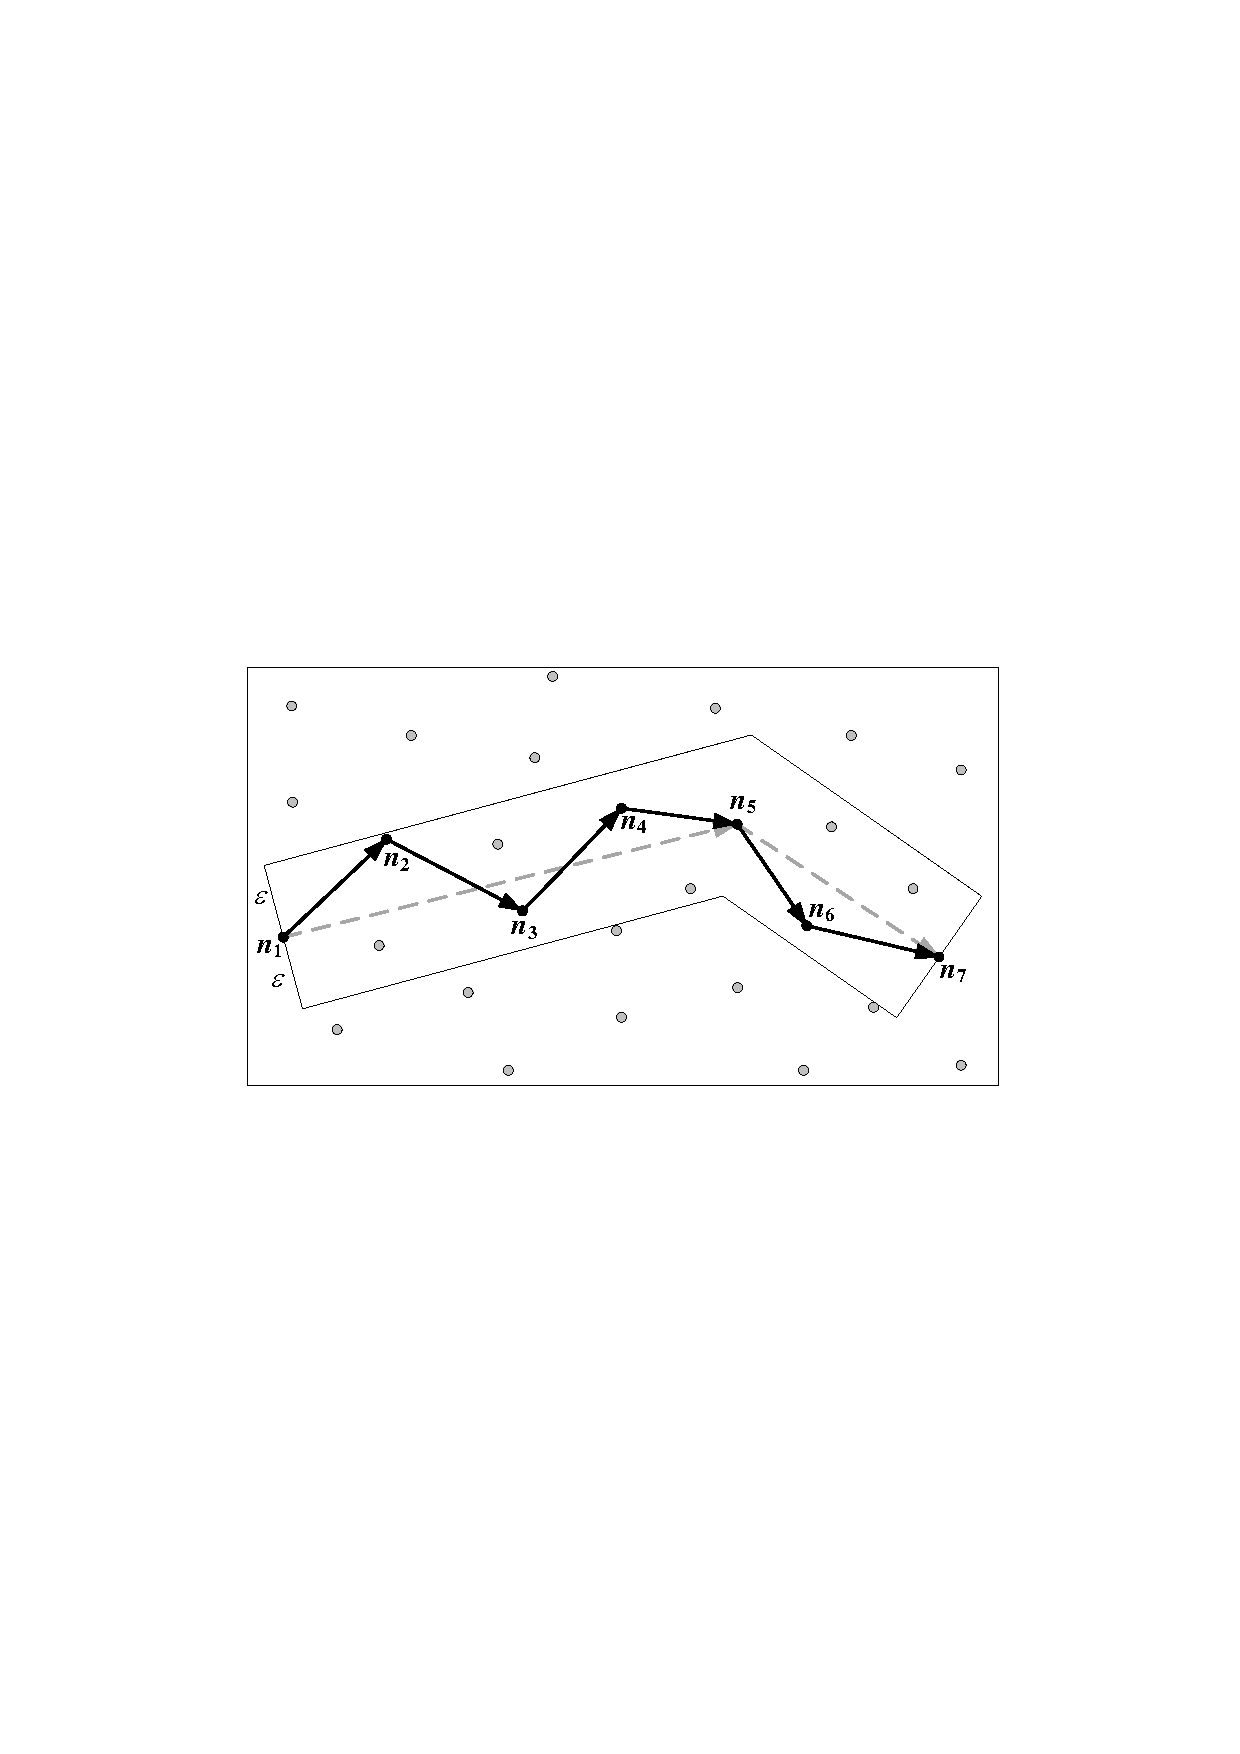
\includegraphics[width=.45\textwidth]{fig504-a}}\hspace{2em}
  \subfloat[虚拟路径无须由真实节点构成]{
    \label{fig:504b}
    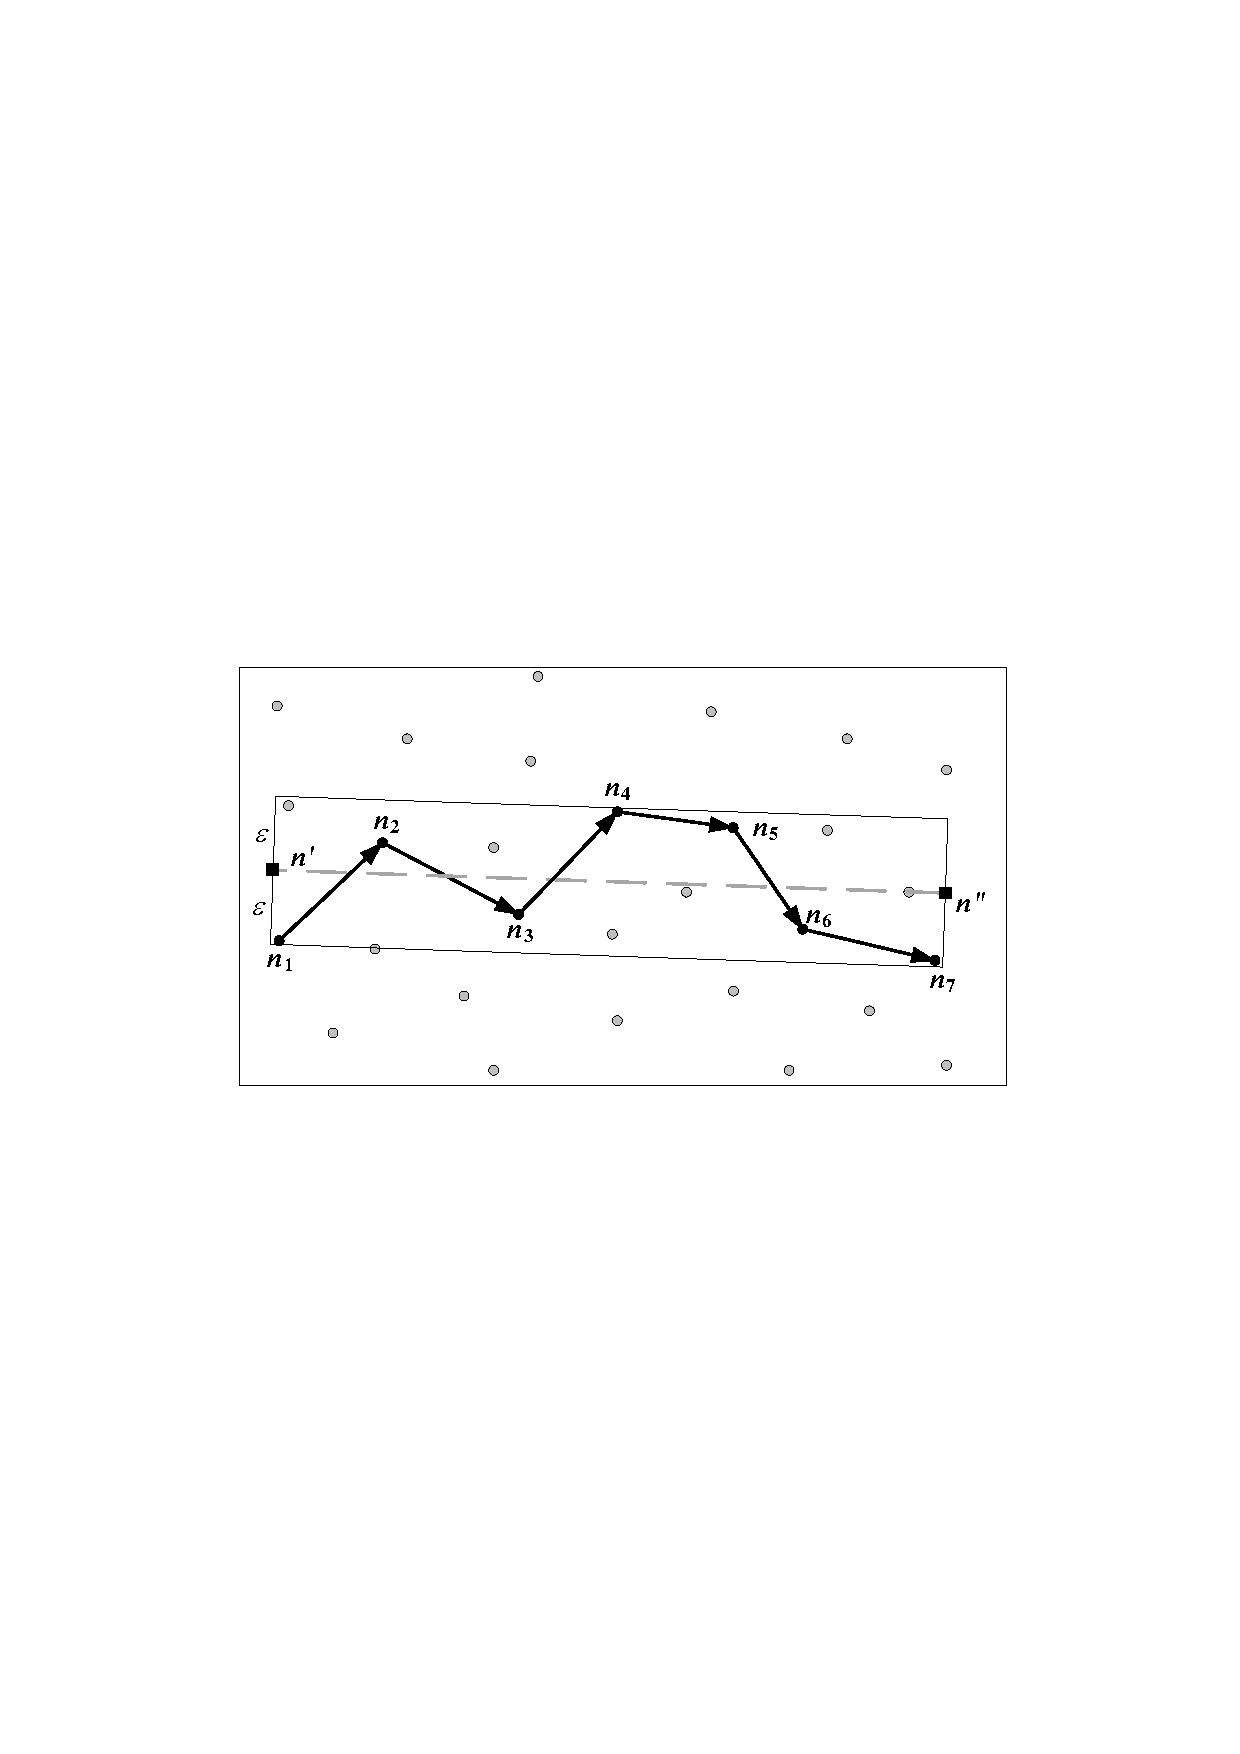
\includegraphics[width=.45\textwidth]{fig504-b}}
  \caption{两种虚拟路径机制的示例}
  \label{fig:504}
\end{figure}

目前已经有大量的PLA算法被广泛应用于不同的研究领域。结合文献\upcite{datamining}中的介绍,本章将这些算法分为两种:在线(online)算法和离线(offline)算法。大部分的在线算法都是基于滑动窗口方法(sliding windows method),其基本思想是在保持误差上限的基础上,贪婪地用每根虚拟线段近似尽可能多的点。离线的PLA算法分为两种:自上而下(top-down)的算法和自下而上(bottom-up)的算法。自上而下的算法迭代地对所有点进行分割直到达到误差上限。自下而上的方法从一个初始化状态开始,按照一定的原则将相邻的线段合并直到达到误差上限。设计PLA算法时需要考虑的另外一个重要因素是,虚拟线段的端点是否必须是原始数据中实际的点。具体到虚拟路径问题中就是,虚拟路径中记录的点是否必须是真实的节点。图\ref{fig:504a}和图\ref{fig:504b}分别代表了这两种情况,其中图\ref{fig:504a}表示虚拟路径必须由真实节点构成,而图\ref{fig:504b}表示虚拟路径无需由真实节点构成。可见,后者得到的虚拟路径包含更少的节点,这一结果在文献\upcite{optimal_PLA}中也得到了证明。文献\upcite{plamlis}将离散域中的PLA问题建模为最短路径问题,并提出了多项式时间算法来求得最优解。算法在最差情况下的复杂度为$O(n^2)$,其中$n$表示点的数量。但是,该算法是集中式的,且计算复杂度对于资源受限的传感器节点来说太高。

本章提出了一种轻量级的在线的PLA算法来解决虚拟路径问题,称为PLA-VP。PLA-VP基于滑动窗口方法,误差函数定义为真实路径中的节点与虚拟路径中的近似线段(或其延长线)之间的垂直距离。另外,算法选择真实节点作为虚拟路径的点,其原因包括两个方面:第一,直接选择实际节点作为虚拟路径中近似线段的顶点,可以有效地降低算法的计算量;第二,从平面中选择任意的坐标点作为近似线段的顶点,虽然能得到更少的虚拟线段,但这些虚拟线段很可能是不连续的,因此记录这些虚拟线段往往需要更多的坐标点。例如,描述$m$条连续的线段只需要$m+1$个点,而描述$m$条独立的线段则需要$2m$个点。利用以上的算法设计原则,对图\ref{fig:504a} 中所示的路径${\{n_1,n_2,n_3,n_4,n_5,n_6,n_7\}}$进行处理,就可以得到其虚拟路径${\{n_1,n_5,n_7\}}$,同时满足公式\ref{equ:602}中所示的条件,其中$seg(n_i,n_j)$表示顶点$n_i$和$n_j$连成的线段,$dist(n_i,seg(n_j,n_k))$表示点$n_i$到线段$seg(n_i, n_j)$或其延长线的垂直距离,$\varepsilon$表示距离误差的上限。
\begin{equation}\label{equ:602}
\left\{\begin{array}{ll}
dist_{i={2,3,4}}(n_i,seg(n_1,n_5))\leq\varepsilon\\
dist_{i={6}}(n_i,seg(n_5,n_7))\leq\varepsilon
\end{array} \right.
\end{equation}

下面结合实际的数据包发送过程,描述算法的具体执行过程。首先,统一地将数据包的源节点$n_{source}$标记为虚拟路径中第一个点。数据包到达第一个中继节点$n_{source}^1$后,算法将线段$seg(n_{source}, n_{source}^1)$标记为当前的近似线段。随后,数据包每到达一个新的中继节点$n_{source}^i$,算法将当前的近似线段更新为$seg(n_{source},n_{source}^i)$,并计算之前的所有中继节点$(n_{source}^1,\ldots,n_{source}^{i-1})$到当前的近似线段的垂直距离。如果有节点到当前的近似线段的垂直距离大于误差上限值$\varepsilon$,则将节点$n_{source}^{i-1}$加入虚拟路径中。随后,算法将虚拟路径中的最后一个节点(如$n_{source}^{i-1}$)作为新的起始节点,并重复以上过程,直到数据包被发送至基站。

目前为止,算法仍存在一个局限,即数据包每到达一个新的节点,都需要计算之前的所有中继节点到当前的虚拟线段的距离,因此必须在数据包中记录之前的所有中继节点的坐标信息。显然,这些计算和存储开销对于传感器节点来说都是过高的。另外,由于每个数据包的存储空间受限,使得能够保存的中继节点的信息受限,因次每条近似线段能够近似的节点的数量受限,虚拟路径的压缩率也将受限。为了解决这一问题,我们引入了范围角(zone angle)方法\upcite{ZoneAngle},如定义\ref{def:503}所示。
\begin{definition}\label{def:503}
对于任意两个坐标为$(x_i,x_j)$和$(x_j,y_j)$的点$i$和$j$,以及给定的误差上限$\varepsilon$,点$j$相对于点$i$的范围角定义为以点$i$为顶点,以$seg(i,j)$为平分线,度数为$2\arcsin(\varepsilon/\sqrt{(y_j-y_i)^2+(x_j-x_i)^2})$的角,表示为$\theta_{(i,j)}^{\varepsilon}$。
\end{definition}

\begin{figure}[h]
\centering
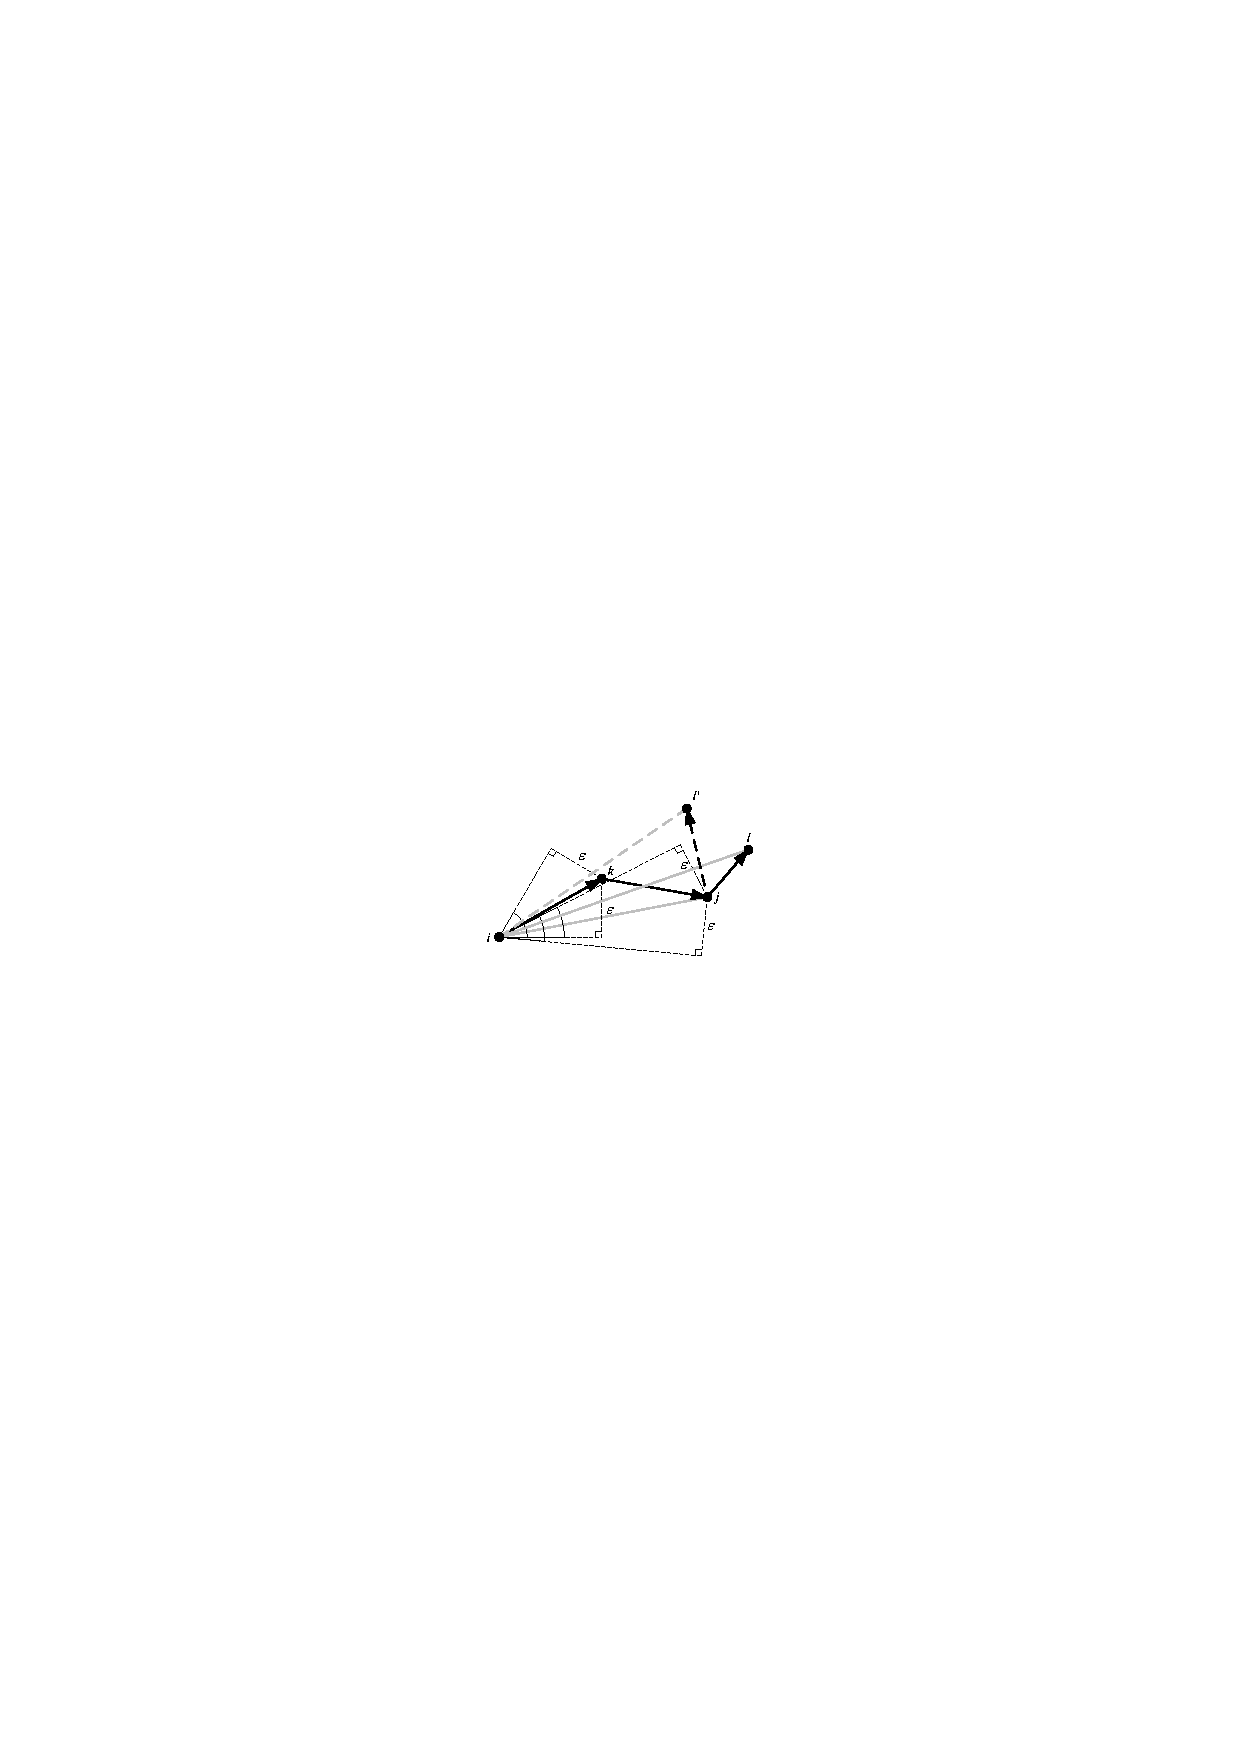
\includegraphics[width=0.6\textwidth]{fig505}
\caption{范围角的定义示意图}
\label{fig:505}
\end{figure}
PathZip-G利用范围角的基本思想与文献\upcite{ZoneAngle}中相似,但采用了不同的误差测量函数。如图\ref{fig:505}所示,对于点$j$,如果线段$seg(i,j)$落在范围角$\theta_{(i,k)}^{\varepsilon}$内,则点$k$到线段$seg(i,j)$的垂直距离一定不大于$\varepsilon$,也就是说点$k$可以用线段$seg(i,j)$来近似。这一结果可以进一步地扩展到包含多个节点的情况,如果点$l$落在点$k$和$j$的范围角的重叠区域$\theta_{(i,k)}^{\varepsilon}\cap{\theta_{(i,l)}^{\varepsilon}}$内,则点$k$和点$j$均可以用线段$seg(i,l)$来近似。而点$l^{'}$不在$k$和$j$的范围角的重叠区域,所以点$k$和$j$不能同时地用线段$seg(i,l^{'})$来近似。基于以上原理,我们给出了定理\ref{theorem501}。
\begin{theorem}
  \label{theorem501}
给定误差上限$\varepsilon$和三个点$n_i$,$n_j$,$n_k$,当且仅当线段$seg(n_i,n_k)$落在点$n_j$的范围角$\theta_{(i,j)}^{\varepsilon}$内时,点$n_j$可以用线段$seg(n_i,n_k)$来近似。
\end{theorem}
\begin{proof}
首先证明其充分性。如果线段$seg(n_i,n_k)$落在点$n_j$的范围角$\theta_{(i,j)}^{\varepsilon}$内,则线段$seg(n_i,n_k)$与点$j$的范围角的中分线$seg(i,j)$之间的夹角$\alpha$一定满足$\alpha<\arcsin(\varepsilon/\sqrt{(y_j-y_i)^2+(x_j-x_i)^2})$,所以点$j$到线段$seg(n_i,n_k)$的垂直距离一定满足$l<\sin{(\arcsin(\varepsilon/\sqrt{(y_j-y_i)^2+(x_j-x_i)^2}))}\times\sqrt{(y_j-y_i)^2+(x_j-x_i)^2}=\varepsilon$,则点$n_j$可以被线段$seg(n_i,n_k)$近似。必要性的证明过程与之相反,这里不再赘述。
\end{proof}

将定理\ref{theorem501}扩展至一般的情况,可以得到定理\ref{theorem502}。
\begin{theorem}
  \label{theorem502}
给定误差上限$\varepsilon$、起始点$n_{start}$,以及一组中继节点$(n_i,\ldots,n_k,\ldots,n_j)$,对于任意一个新的点$n_{new}$,当且仅当线段$seg(n_{start},n_{new})$落在中继节点的范围角的重叠区域$\bigcap_{l=i}^{j}\theta_{(start,i)}^{\varepsilon}$中时,所有的中继节点都能用线段$(n_{start},n_{new})$来近似。
\end{theorem}
\begin{proof}
首先证明其充分性。如果线段线段$seg(n_{start},n_{new})$落在中继节点的范围角的重叠区域$\bigcap_{l=i}^{j}\theta_{(start,i)}^{\varepsilon}$中,则一定也落在每一个中继节点的范围角内。那么利用定理\ref{theorem501}就可以很容易地判断每一个中继节点都可以用线段$(n_{start},n_{new})$来近似。必要性的证明过程与之相反,这里也不再赘述。
\end{proof}

\begin{algorithm}[t]
\caption{虚拟路径算法PLA-VP}
\label{alg:502}
\begin{algorithmic}[1]
\REQUIRE ~~\
实时产生的路径$P$,误差上限$\varepsilon$
\ENSURE ~~\
虚拟路径$P^{'}$
\STATE 初始化虚拟路径为$P^{'}:=\phi$;                                                          \label{alg:502:01}
\STATE 初始化起始节点为$n_{start}:=n_{source}$;                                                \label{alg:502:02}
\STATE 初始化范围角为$\theta_{overlap}:=\theta_{(start,1)}^{\varepsilon}$;                     \label{alg:502:03}
\WHILE {$n_{new}\neq{\phi}$}                                                                    \label{alg:502:04}
    \IF {$seg(n_{start},n_{new})$落在$\theta_{overlap}$内}                                      \label{alg:502:05}
        \STATE 计算$n_{new}$的范围角$\theta_{(start,new)}^{\varepsilon}$;                      \label{alg:502:06}
        \STATE $\theta_{overlap}:=\theta_{(start,new)}^{\varepsilon}\land{\theta_{overlap}}$;  \label{alg:502:07}
    \ELSE                                                                                       \label{alg:502:08}
        \STATE 将$n_{new-1}$加入虚拟路径$P^{'}$中;                                             \label{alg:502:09}
        \STATE 更新起始节点为$n_{start}:=n_{new-1}$;                                           \label{alg:502:10}
        \STATE 计算$n_{new}$的范围角$\theta_{(start,new)}^{\varepsilon}$;                      \label{alg:502:11}
        \STATE $\theta_{overlap}:=\theta_{(start,new)}^{\varepsilon}$;                         \label{alg:502:12}
    \ENDIF                                                                                      \label{alg:502:13}
\ENDWHILE                                                                                       \label{alg:502:14}
\STATE 将汇聚节点$n_{sink}$加入虚拟路径$P^{'}$中,输出$P^{'}$;                                 \label{alg:502:15}
\end{algorithmic}
\end{algorithm}
根据定理\ref{theorem501}和定理\ref{theorem502},我们只需要在数据包中保存中继节点的范围角重叠区域。数据包到达一个新的节点后,算法通过检验该节点是否落在重叠区域就可以判断该节点是否可以用当前的虚拟线段来近似。至此,我们得到了完整的虚拟路径算法PLA-VP,如算法\ref{alg:502}所示。在该算法中,每个节点只需要计算一次范围角,而且每个数据包中只需要记录范围角的重叠区域。因此,算法\ref{alg:502}具有线性计算复杂度$O(n)$,以及常数存储开销$O(1)$,其中$n$表示路径中节点的数量。
\section{实验评估}
本节通过大量的仿真实验验证PathZip及PathZip-G在不同网络条件下的性能。实验主要对两个性能指标进行评估,分别是算法的压缩率和计算复杂度,并对几个主要的参数对算法性能的影响进行验证。
\subsection{实验设置}
在整个仿真实验中,仿真网络的节点数量在100至10000的范围变化,网络部署区域为一个正方形的平面。在实验过程中还采用了其它多种不同形状的网络,并得到了一致的结果,本章中由于篇幅的限制不再赘述。为了便于生成网络拓扑,本章采用Q-UDG模型构建网络连通图。为了评估算法在不同节点密度下的性能,本章通过调整节点的通讯半径来改变网络的平均节点度。本章假设记录每个节点ID需要2字节的存储开销,也就是说网络中最大支持$2^{16}$个节点,完全能够满足大规模网络的需求。在整个仿真实验中,每一项测试都对100个独立、随机生成的网络进行测试并给出平均值。
\subsection{PathZip方法评估}
下面对PathZip方法的主要性能指标进行评估,分别是压缩率、计算复杂度,以及SPH哈希函数的抗冲突性。本节中压缩率表示为记录初始的路径信息需要的存储开销与基于哈希的路径路径记录方法的存储开销的比值,计算复杂度表示恢复路由路径需要进行哈希计算的候选路径的数量。
\subsubsection{压缩率}
首先评估PathZip方法的压缩率,并与之前的LZW压缩算法进行比较。

对于不同的路径长度,我们分别随机地从网络中选择1000条路径,利用PathZip和LZW算法对这些路径进行处理,并计算存储开销的平均值以及对应的压缩率。实验结果如图\ref{fig:506}所示。
\begin{figure}[t]
  \centering
  \subfloat[压缩率]{
    \label{fig:506a}
    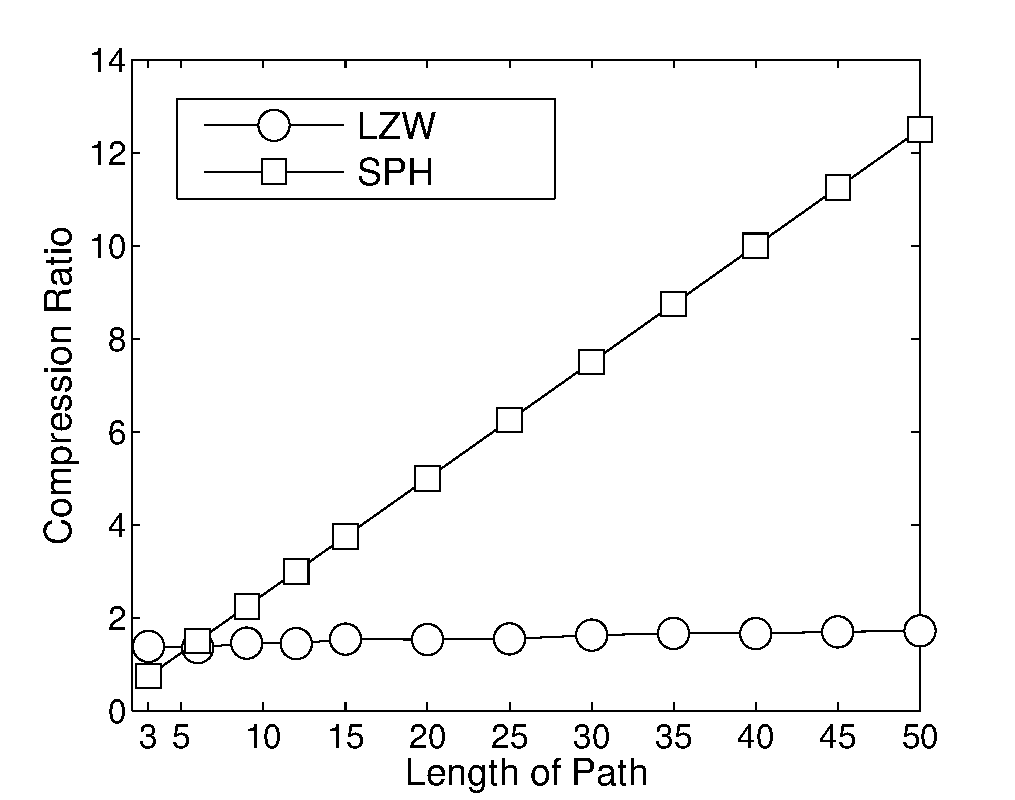
\includegraphics[width=.45\textwidth]{fig506-a}}\hspace{0.5em}
  \subfloat[存储开销]{
    \label{fig:506b}
    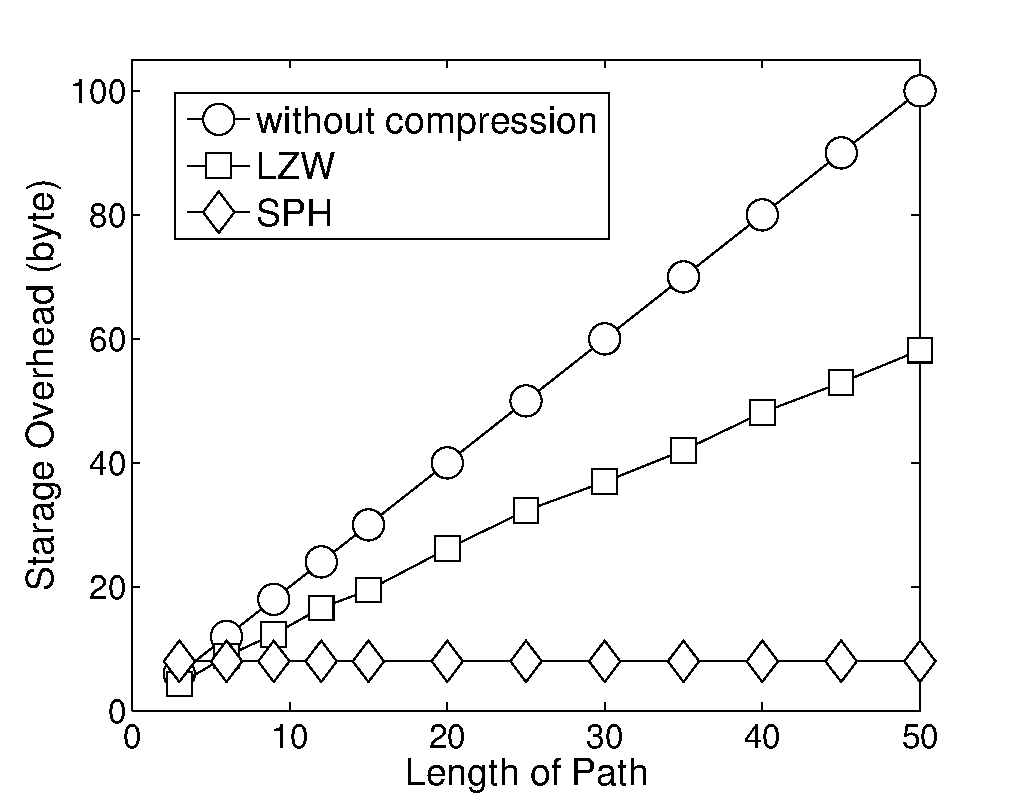
\includegraphics[width=.45\textwidth]{fig506-b}}
  \caption{PathZip的压缩率和存储开销}
  \label{fig:506}
\end{figure}

在图\ref{fig:506a}中,$x$轴表示路径的平均长度,$y$轴表示两种方法对不同长度的路径的压缩率。从实验结果可以看出,PathZip方法的压缩率随着路径长度的增加而线性增长。这是由于PathZip将任意长度的路由路径压缩成固定长度的输出(即64位的哈希值),显然其压缩率将随着输入数据量的增加而线性增长,这也是理论上能够获得的最优的压缩率。作为对比,我们基于LZW压缩算法构造了另一种路径压缩算法。数据包的源节点调用LZW压缩算法将自己的ID进行压缩,并存储在数据包中。对随后,数据包每到达一个新的节点,首先对储存的压缩路径信息进行解压,将本节点的ID附加在解压后的数据中并重新进行压缩。新的压缩结果作为新的路径压缩信息被保存在数据包中。我们仍然用LZW表示这一构造出的路径压缩算法。图\ref{fig:506a}中结果显示LZW的压缩率随着路径长度的增加而缓慢地增长。具体来讲,LZW对3 跳路径的平均压缩率为1.38,对30跳路径的平均压缩率为1.62,而对50跳以上路径的压缩率依然稳定在1.8以下。可见,PathZip在压缩率方面,相对于LZW算法具有明显的优势。

为了更直观地表示PathZip在存储开销方面的优势,下面对两种方法的存储开销进行比较。在图\ref{fig:506b}中,$x$轴表示路径的平均长度,$y$轴表示两种方法记录不同长度的路径的存储开销。从实验结果可以看出,LZW算法的存储开销随着路径长度的增加呈线性增长,使得其在大规模网络中的可用性受限。相对地,PathZip方法仅需要较低且始终恒定的存储开销,因此在大规模网络中具有非常好的可用性和可扩展性。
\subsubsection{计算复杂度}
PathZip方法的计算开销主要包括两个部分,第一部分来自于节点端的哈希计算,第二部分来自于基站端的路径验证过程。哈希计算是固定的常数开销,本章前面已经进行了介绍。下面通过仿真实验对第二部分的计算开销进行评估,实验结果如图\ref{fig:507}所示。
\begin{figure}[t]
  \centering
  \subfloat[计算复杂度上限]{
    \label{fig:507a}
    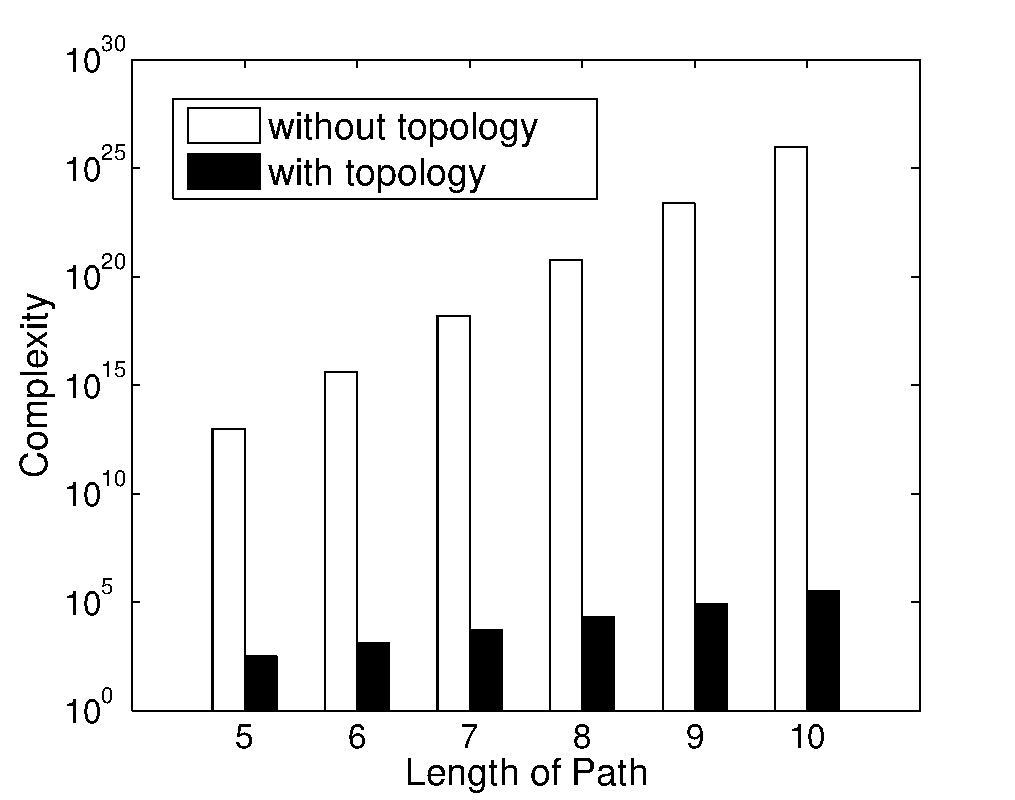
\includegraphics[width=.45\textwidth]{fig507-a}}\hspace{0.5em}%
  \subfloat[节点密度的影响]{
    \label{fig:507b}
    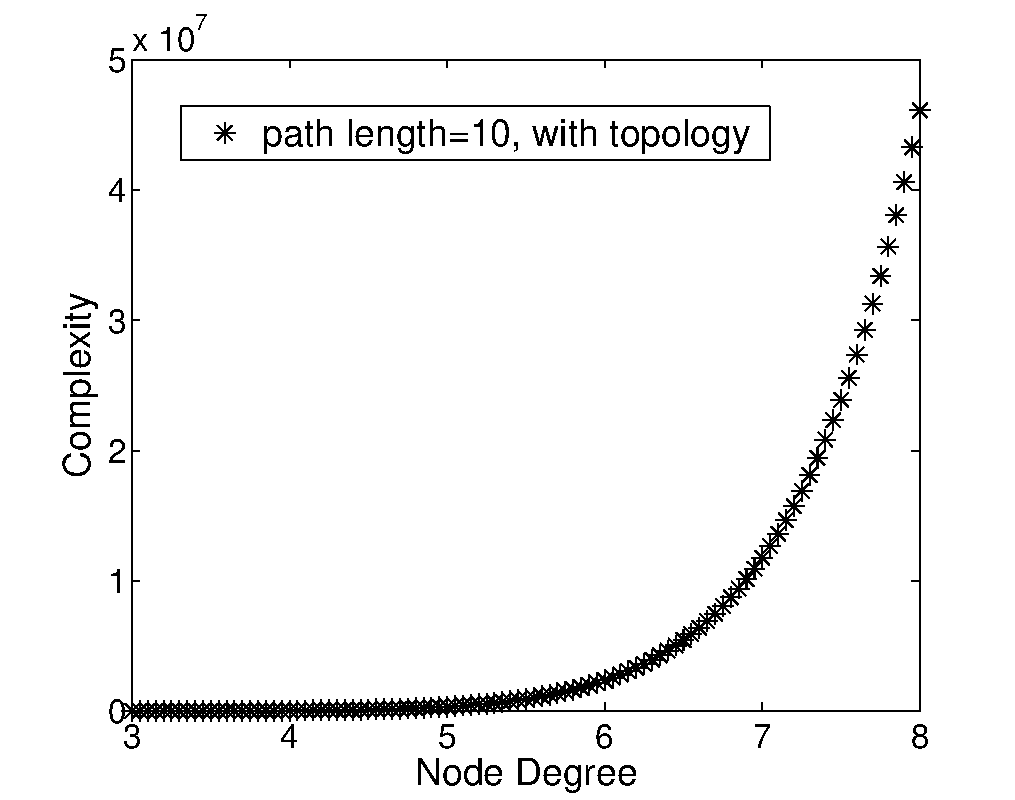
\includegraphics[width=.45\textwidth]{fig507-b}}\hspace{0.5em}%
  \subfloat[实际的计算复杂度]{
    \label{fig:507c}
    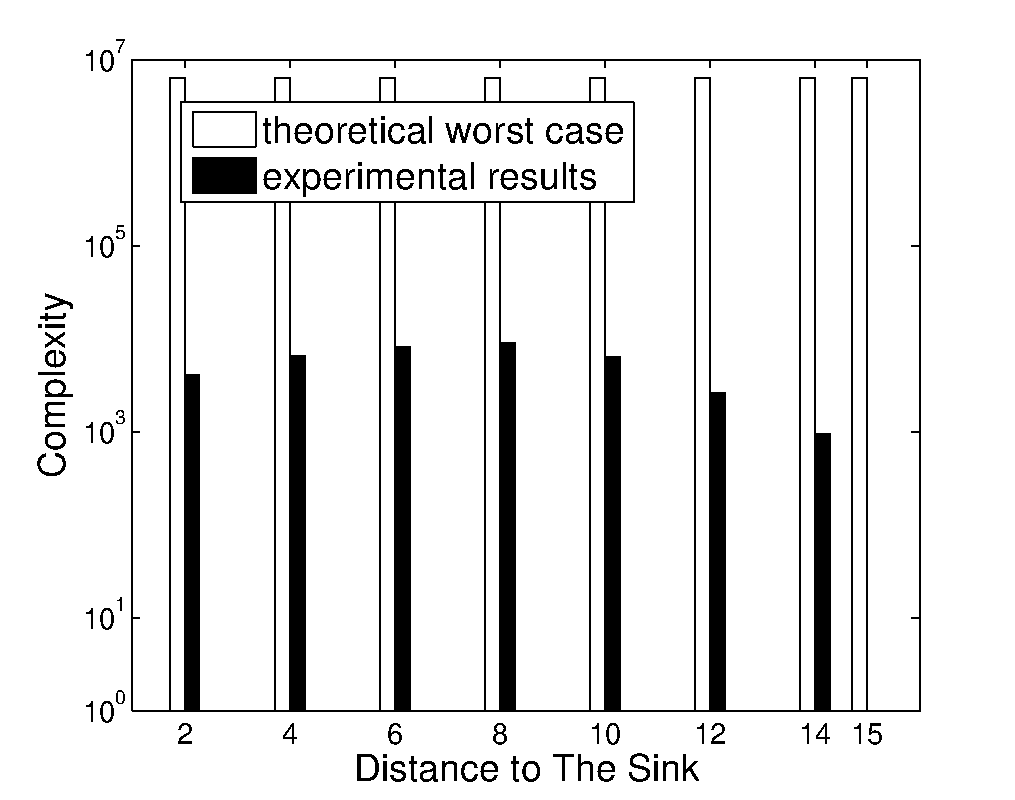
\includegraphics[width=.45\textwidth]{fig507-c}}\hspace{0.5em}%
  \subfloat[路径数量与长度的关系]{
    \label{fig:507d}
    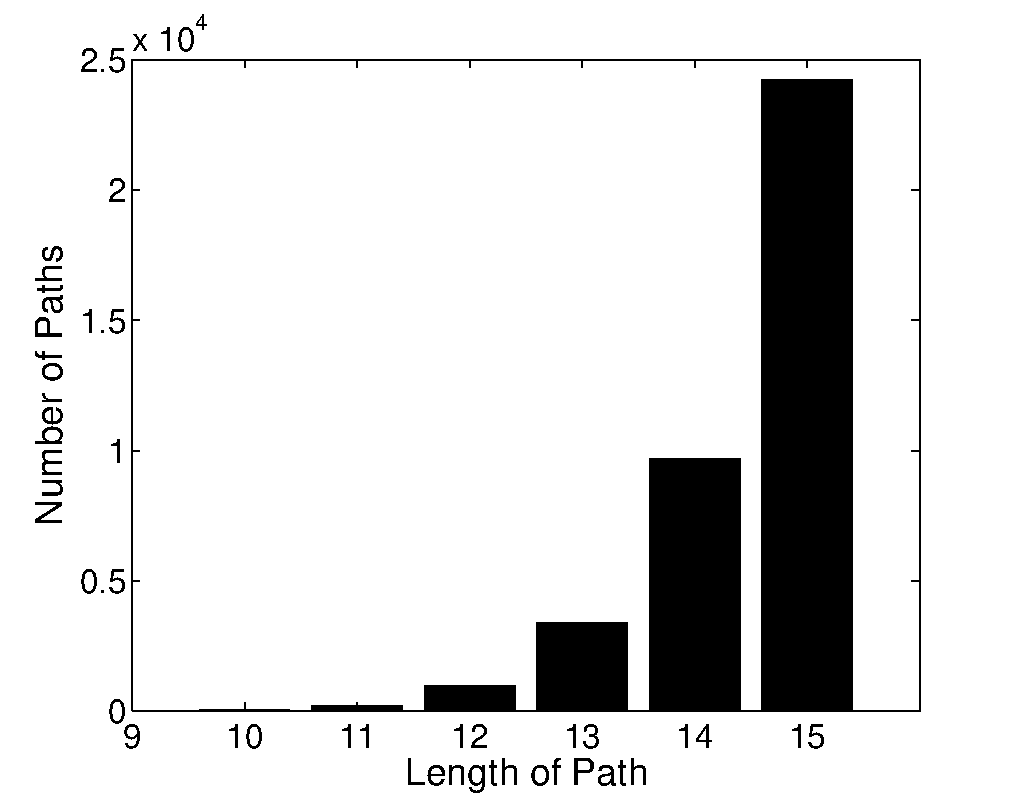
\includegraphics[width=.45\textwidth]{fig507-d}}
  \caption{PathZip的计算复杂度}
  \label{fig:507}
\end{figure}

在不利用任何拓扑信息的情况下,路径验证过程的开销非常高甚至是无法接受的。首先,我们对利用拓扑信息前后,算法的计算复杂度的理论值进行比较。在图\ref{fig:507a}中,$x$轴表示路径的长度,$y$轴表示对于不同长度的路径,在利用拓扑信息前后,需要进行哈希计算的候选路径的数量的上限值,其中网络的平均节点度始终为5。实验结果显示,利用拓扑信息可以显著地降低路径验证过程的计算复杂度。然后,我们评估节点密度对路径验证过程的计算复杂度上限的影响,如图\ref{fig:507b}所示,其中$x$轴表示平均节点度,$y$轴表示对于不同的平均节点度,验证一条10跳路径的计算复杂度的上限。可见,随着节点度的增加,计算复杂度的上限值也快速地提高。

前面评估了算法在理论最差情况下的计算复杂度,而实际的实验结果要远远优于理论最差情况。对于网络中的每个节点,我们计算出该节点到基站的所有的14跳路径的数量,将其与理论最差情况下的计算复杂度进行比较。该组实验采用的网络中包含400个节点,部署在正方形区域中,平均节点度为4,基站位于部署区域的中心位置。实验结果如图\ref{fig:507c}所示,其中$x$轴表示节点到基站的最短距离,$y$轴表示节点到基站的所有的14跳路径的数量。可见,实际实验中的计算复杂度远远低于理论最差情况。从图中所示的结果中,我们还观察到另外一个有趣的现象,即计算复杂度首先随着节点到基站的最短距离的增加而增加;而在最短距离达到一定的值之后,计算复杂度反而随着最短距离的增加而降低。下面对产生这一现象的原因进行分析。当源节点距离基站较近时,该源节点至基站的14跳路径可以从基站的各个方向到达基站。此时,当源节点与基站的距离增加时,将会有更多的中继节点可以选择,因此可选路径的数量也相应地增加。当源节点到基站的距离增加至一定的值之后,路径可以到达基站的方向角随着距离的增加而减小,因此可选路径的数量也相应地减少。

另外,PathZip在几何贪婪的路由协议下(如最短路径路由)的计算复杂度较低。这是因为节点到基站的最短路径的数量比更长路径的数量要少。下面通过仿真实验来验证这一猜想。我们从网络中找出所有的距离基站的最短路径长度为10的节点,并分计算其它的指定长度的路径的平均数量。实验结果如图\ref{fig:507d}所示,其中$x$ 轴表示路径长度,$y$轴表示不同长度路径的数量的平均值。实验结果显示,路径的数量随着路径长度的增加而快速地增加,如长度为10的最短路径的数量为20.8,而长度为12的路径的数量为940。
\subsubsection{SPH的抗冲突性}
下面对SPH哈希函数的抗冲突性进行评估。实验采用四个节点数量分别为100、400、900、1600的网络,平均节点度均为4.8,基站位于正方形部署区域的中心位置。然后,我们从每个网络中找出所有节点至基站的最短路径,并利用SPH哈希函数对这些路径的哈希值进行计算。表\ref{table501}给出了四个网络中所有最短路径的数量以及每个网络中这些路径的哈希值出现冲突的次数。结果显示,在四个网络中均没有出现冲突。
\begin{table}[h]
\caption{不同规模的网络中冲突路径的数量}
\label{table501}
\centering
\begin{tabular}{ccc}
\toprule[1.5pt]
{\hei 节点数量} & {\hei 最短路径的数量} & {\hei 冲突的数量}\\\midrule[1pt]
100 & 404 & 0     \\ \midrule[1pt]
400 & 9831 & 0    \\ \midrule[1pt]
900 & 120446 & 0  \\ \midrule[1pt]
1600 & 367142 & 0 \\ \bottomrule[1.5pt]
\end{tabular}
\end{table}

为了增加仿真实验的规模和输入数据的随机性,我们进行了更多的实验。我们随机地构建了322000条不同的路径,每条路径由1-4000的节点ID随机地构成。这些路径包括46 组,每组中的路径具有相同的长度(从5至50)。然后,我们利用SPH哈希函数计算出所有路径的哈希值,并找出出现冲突的次数。在计算结果中,出现冲突的次数仍然为0。因此,我们可以认为SPH对于路由路径记录问题提供了充分的抗冲突性。
\subsection{PathZip-G方法评估}
本节对PathZip-G方法的性能进行评估,主要评测两个性能指标,分别是计算复杂度和压缩率。
\subsubsection{计算复杂度}
PathZip-G的主要目的是进一步降低PathZip的计算复杂度。下面对PathZip-G的计算复杂度进行评估,并与PathZip进行比较。实验结果如图\ref{fig:508}所示。

首先分析PathZip-G在不同的误差上限设置下的计算复杂度。仿真网络部署在圆形区域内,包含2500个节点,平均节点度为5,基站位于部署区域的中心位置,网络的直径(定义为网络中所有节点到基站的最短距离的最大值)为50跳。我们找出所有的到基站最短距离为6的节点,计算这些节点到基站的长度为10的所有路径的数量,并计算其平均值。图\ref{fig:508a}给出了不同的误差上限设置下PathZip-G的计算复杂度,其中$x$轴表示不同的误差上限,单位为节点的通讯半径,$y$轴表示长度为10 的所有路径的数量的平均值。实验结果显示,误差上限越小PathZip-G的计算复杂度越低。这是因为采用更小的误差上限使得生成的近似几何区域更狭窄,因此候选路径的数量越少。另外,为了直观地将PathZip-G与PathZip进行比较,图中也给出了PathZip的结果。可见,PathZip-G能够有效地降低PathZip方法的计算复杂度。具体来讲,在本组实验中PathZip的计算复杂度为4440,而在误差上限设置为节点通讯半径的1/2时,PathZip-G的计算复杂度仅为44.8。

下面评估节点到基站的距离对PathZip-G的计算复杂度的影响。实验网络中包含400个节点,部署在正方形区域中,平均节点度为4,基站位于部署区域的中心位置。我们从网络中找出到基站的最短距离为指定值的所有节点,计算它们到基站的所有10跳路径的数量,并计算平均值。实验结果如图\ref{fig:508b}所示,其中$x$轴表示节点到基站的最短距离,$y$轴表示所有10跳路径的数量的平均值。实验结果显示,PathZip-G的计算复杂度首先随着节点到基站的距离的增加而增加,当最短距离增加至一定的值后,计算复杂度反而随着节点到基站的距离的增加而降低。这一现象与节点到基站的距离对PathZip的计算复杂度的影响是一致的,其原因也是一致的,这里不再赘述。另外,图\ref{fig:508b}所示的结果再次验证了PathZip-G对PathZip的改进作用,同时也验证了误差上限对PathZip-G的计算复杂度的影响。
\begin{figure}[t]
  \centering
  \subfloat[误差上限的影响]{
    \label{fig:508a}
    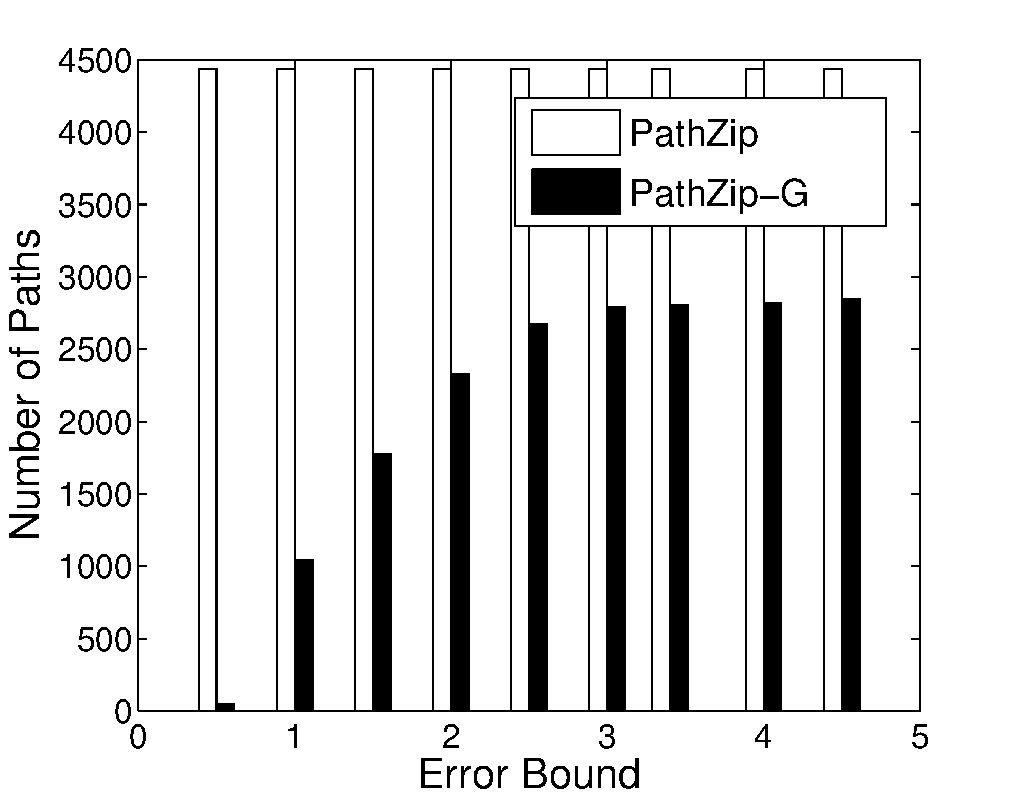
\includegraphics[width=.45\textwidth]{fig508-a}}\hspace{0.5em}
  \subfloat[最短距离的影响]{
    \label{fig:508b}
    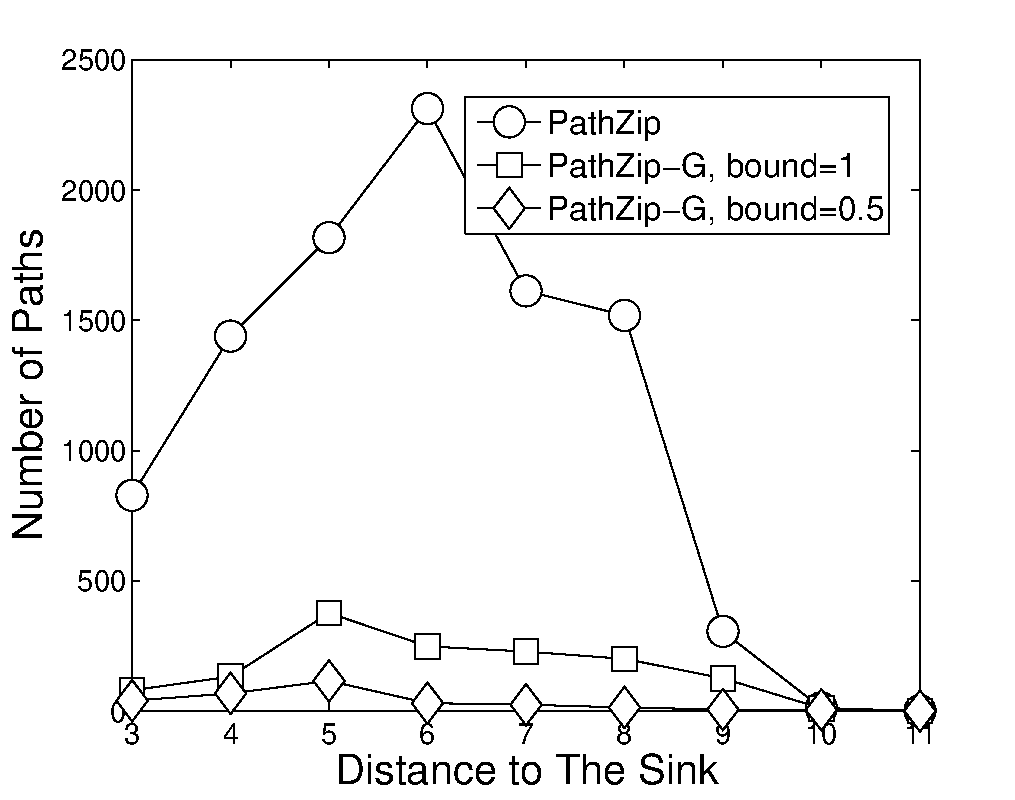
\includegraphics[width=.45\textwidth]{fig508-b}}
  \caption{PathZip-G的计算复杂度}
  \label{fig:508}
\end{figure}

\subsubsection{压缩率}
本节对PathZip-G的压缩率和存储开销进行评估,并分析几个重要的参数对压缩率的影响。本节中的压缩率定义为初始路径的长度与对应的虚拟路径长度之间的比值,存储开销表示数据包保存虚拟路径所需要的存储空间的大小。

1. 误差上限的影响

误差上限是PathZip-G方法中一个关键的参数,显著地影响着基于PLA的虚拟路径算法的各项性能。首先从直观上进行分析,误差上限越小就越容易和频繁地被超出,因此虚拟路径中就会包含更多的节点,压缩率也相应地降低。与此同时,近似几何区域也越狭窄,其中包含的候选节点的数量也越少,因此计算复杂度也越低。
\begin{figure}[h]
\centering
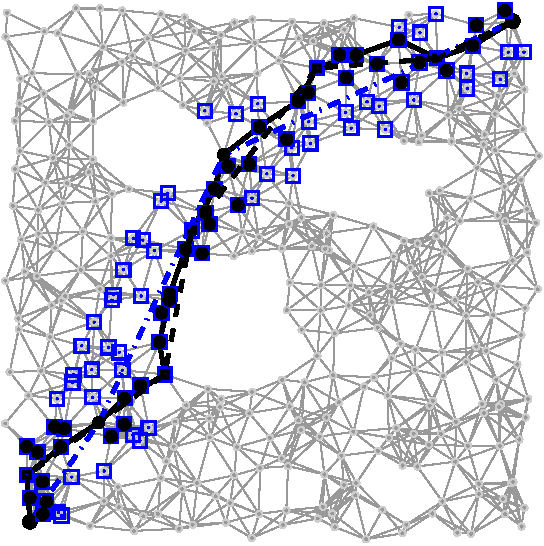
\includegraphics[width=0.55\textwidth]{fig509}
\caption{误差上限对PathZip-G的压缩率的影响}
\label{fig:509}
\end{figure}

下面通过仿真实验来验证以上分析结果。仿真网络包含366个节点,部署在正方形区域中,其网络通讯图如图\ref{fig:509}所示。图中粗实线表示网络中一条20跳的路径。黑色虚线和点表示误差上限为节点通讯半径的1/2时得到的虚拟路径以及对应的候选节点。此时,虚拟路径的压缩率为3,而候选节点的数量为46。蓝色虚线和小正方形表示误差上限为节点通讯半径时得到的虚拟路径以及对应的候选节点。此时,虚拟路径的压缩率为5.25,而候选节点的数量为96。为了更充分地验证以上结果,我们进行了更多的实验,实验结果如图\ref{fig:510a}所示,其中$x$轴表示不同的误差上限,左侧$y$轴表示压缩率,右侧$y$轴表示候选节点的数量。可见,实验结果证实了我们之前的分析结果。更高的压缩率能够节约存储空间,而同时产生的更多的候选节点又会增加路径恢复过程的计算开销。因此,协议设计者需要根据具体应用的需求和系统能力在两者之间进行折中的选择。

2. 网络规模的影响

\begin{figure}[t]
  \centering
  \subfloat[误差上限的影响]{
    \label{fig:510a}
    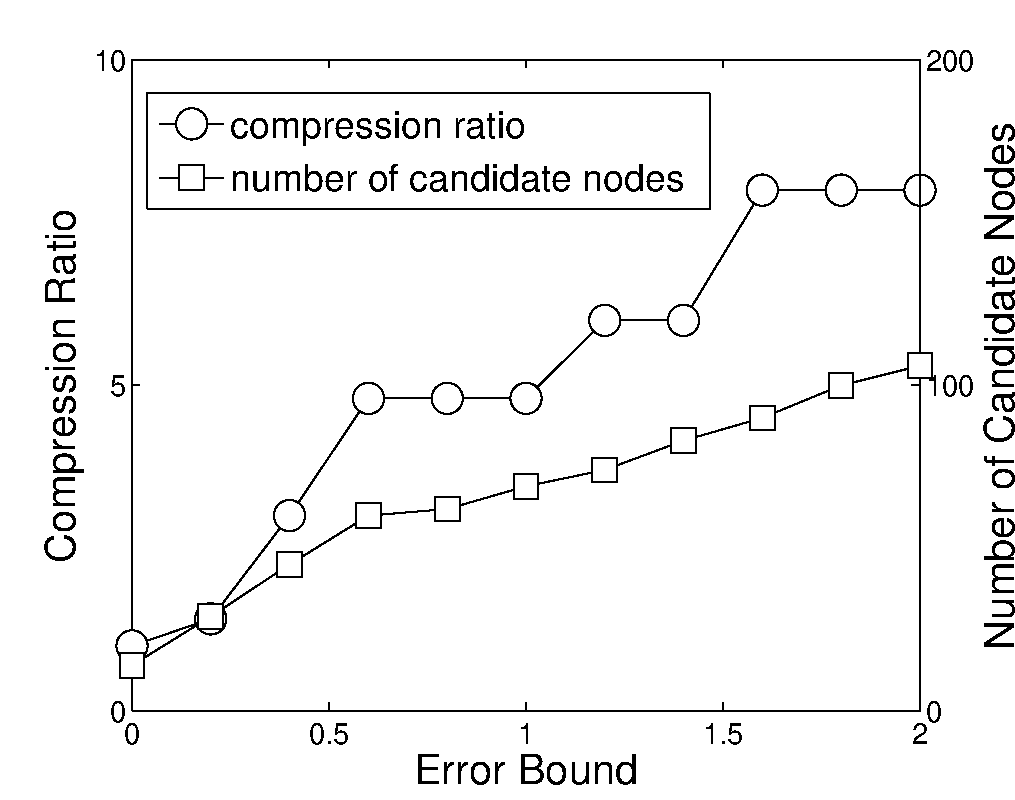
\includegraphics[width=.3\textwidth]{fig510-a}}\hspace{0.5em}
  \subfloat[网络规模的影响]{
    \label{fig:510b}
    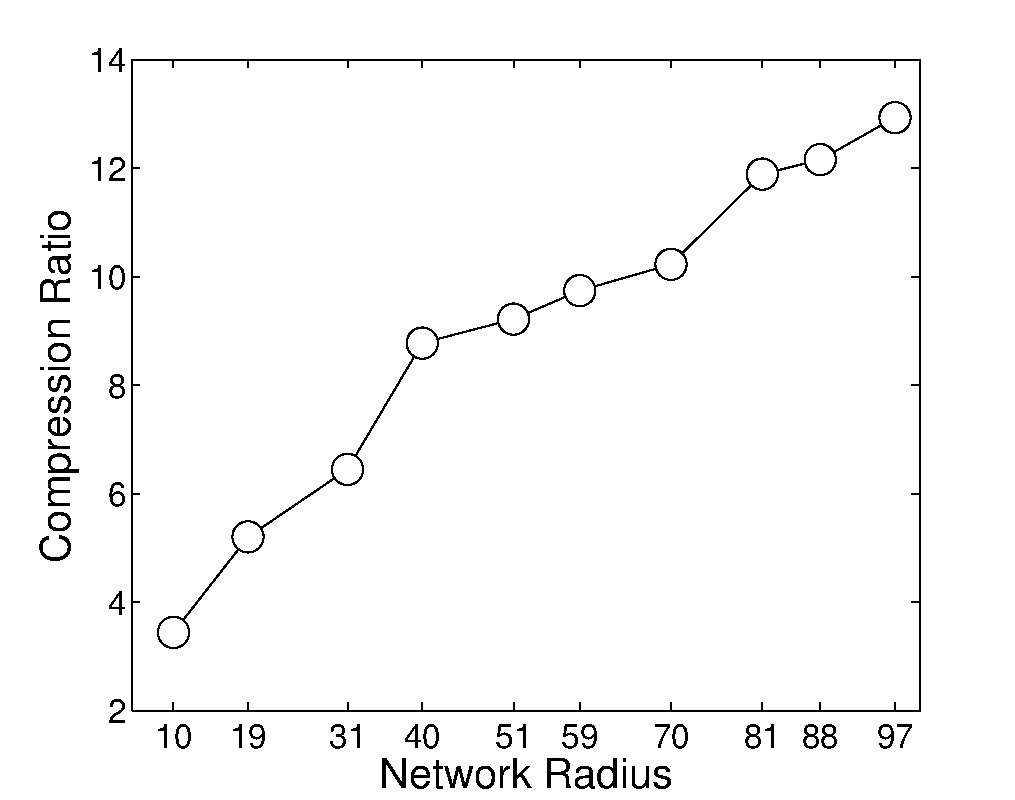
\includegraphics[width=.3\textwidth]{fig510-b}}\hspace{0.5em}
  \subfloat[节点密度的影响]{
    \label{fig:510c}
    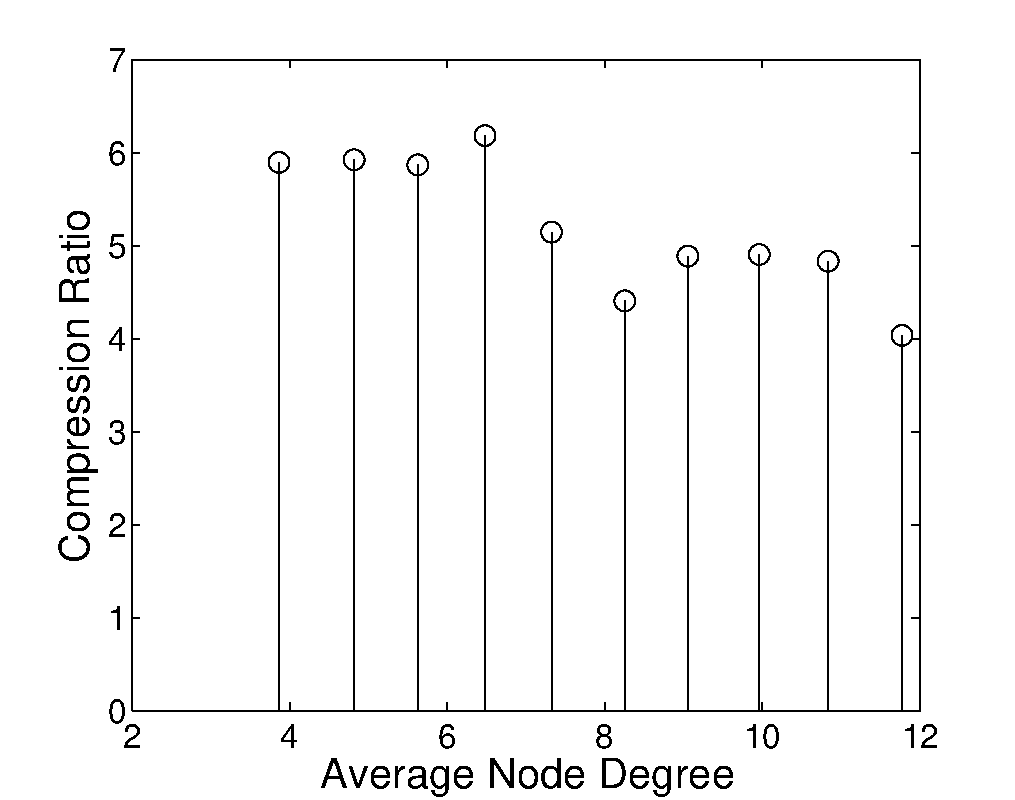
\includegraphics[width=.3\textwidth]{fig510-c}}\hspace{0.5em}
  \subfloat[节点度对路径长度的影响]{
    \label{fig:510d}
    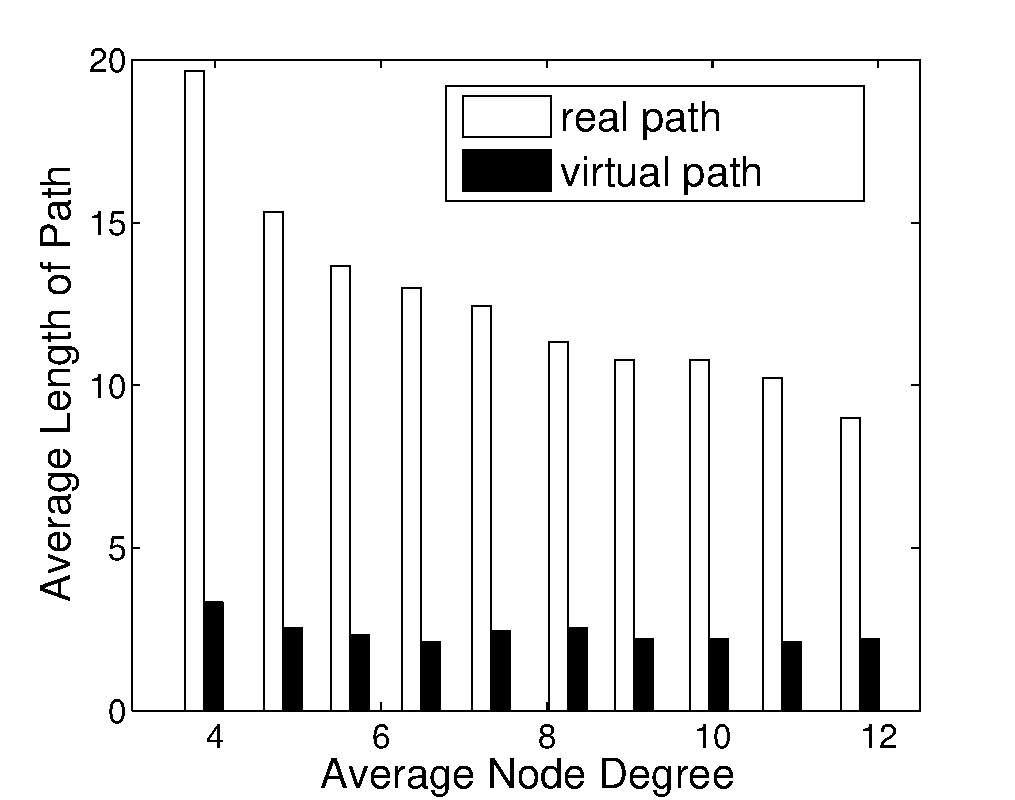
\includegraphics[width=.3\textwidth]{fig510-d}}\hspace{0.5em}
  \subfloat[存储开销]{
    \label{fig:510e}
    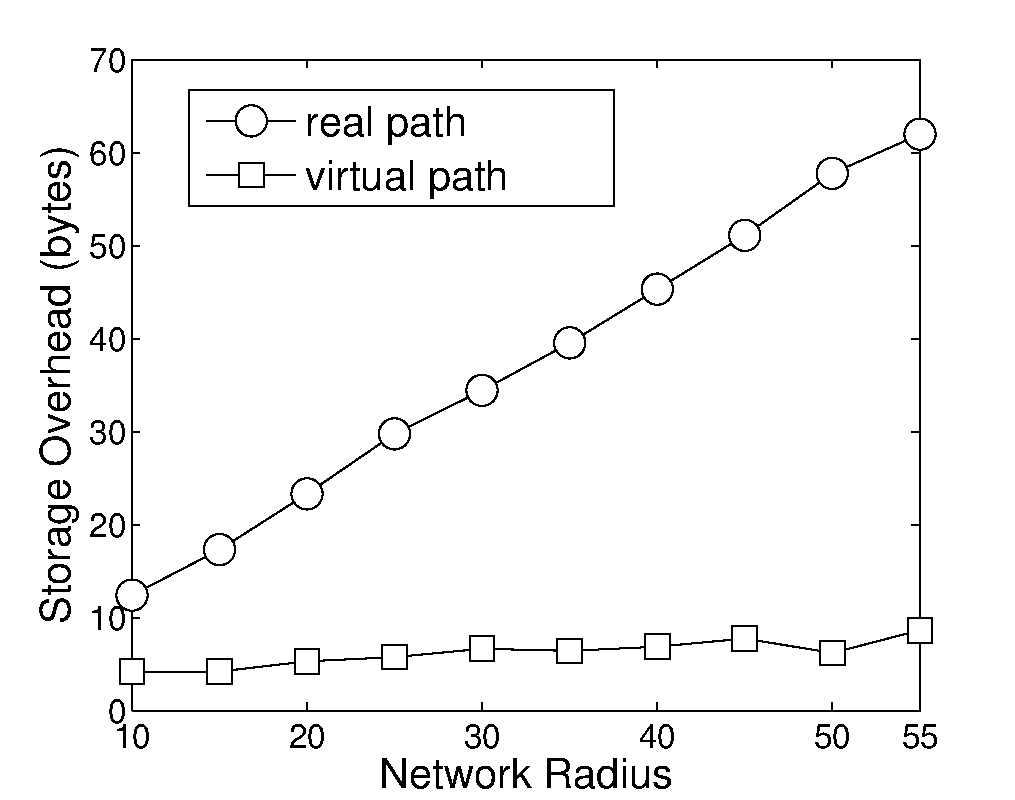
\includegraphics[width=.3\textwidth]{fig510-e}}\hspace{0.5em}
  \subfloat[部署模型的影响]{
    \label{fig:510f}
    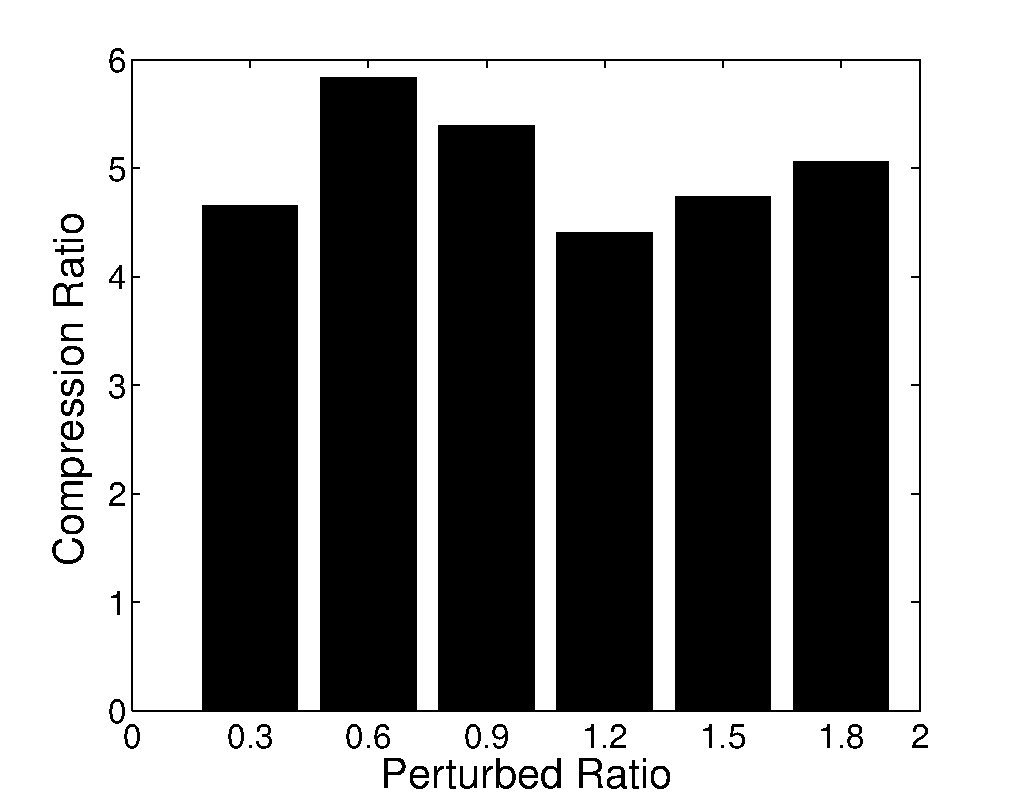
\includegraphics[width=.3\textwidth]{fig510-f}}
  \caption{PathZip-G的压缩率和存储开销}
  \label{fig:510}
\end{figure}
下面评估PathZip-G在不同规模网络中的压缩率。该项性能决定了方法在大规模网络中的可扩展性。

首先,我们构造了不同规模的网络,其节点数量分别是100、400、900、1600、2500、3600、4900、6400、8100、10000,均部署在正方形区域中,基站位于部署区域的中心位置。对于每个网络,我们随机地选择1000个节点对,找出它们之间的最短路径,分别计算对应的虚拟路径的压缩率并计算平均值。在该组实验中,误差上限始终设置为节点的通讯半径。实验结果如图\ref{fig:510b}所示,其中$x$轴表示网络的半径,$y$轴表示不同网络中得到的平均压缩率。可见,PathZip-G的压缩率随着网络规模的增加而显著地提高。下面分析出现这一结果的原因。首先,虚拟路径中始终包含源节点和基站。在规模较小的网络中,实际的路由路径普遍比较短,因此虚拟路径中固有的这两个节点限制了虚拟路径的压缩率。假设网络的直径为10,则由于虚拟路径最短为2,因此压缩率不可能超过5。而在大规模的网络中,由于真实路径的平均长度比较大,这一约束作用将会减弱,而压缩率则相应地提高。因此,PathZip-G在大规模网络中具有良好的可扩展性。

3. 网络密度的影响

下面评估网络密度对PathZip-G方法的压缩率的影响。

仿真网络包含400个节点,部署在正方形区域中,基站位于部署区域的中心位置。首先,我们随机地从网络中选择1000个节点对,找出它们之间的最短路径,分别计算其对应的虚拟路径的压缩率,并计算平均值。然后,我们通过改变节点的通讯半径来调节网络的平均节点度,并分别计算其平均压缩率。在本组实验中,误差上限始终设置为节点通讯半径的1/2。实验结果如图\ref{fig:510c}所示。可见,压缩率随着节点度的增加而缓慢的降低。这是因为,随着平均节点度的增加,节点之间最短路径的长度降低。图\ref{fig:510d}所示的实验结果证明了这一现象,即随着平均节点度的增加,网络中节点之间的最短路径长度的平均值以及对应的虚拟路径长度的平均值均减小。基于前面对网络规模影响的分析结果,压缩率将随着路径长度的减小而降低。因此,压缩率将随着网络密度的增加而降低。

4. 存储开销

下面评估PathZip-G方法在不同规模网络中的存储开销。

首先,我们构造出多个具有不同网络半径的网络,从每个网络中随机地选择1000个节点对,找出它们之间的最短路径,分别计算对应的虚拟路径所需要的存储开销。在本组实验中,误差上限始终设置为节点的通讯半径。实验结果如图\ref{fig:510e}所示,其中$x$轴表示网络的半径,$y$轴表示平均的存储开销。结果显示,PathZip-G 的存储开销随着网络规模的增加而缓慢地增加。例如,网络半径为10时平均存储开销为4.2字节,网络半径增加为55时平均存储开销仅增加至8.6字节。因此,从存储开销的角度看,PathZip-G方法具有非常好的可扩展性。
\begin{figure}[h]
\centering
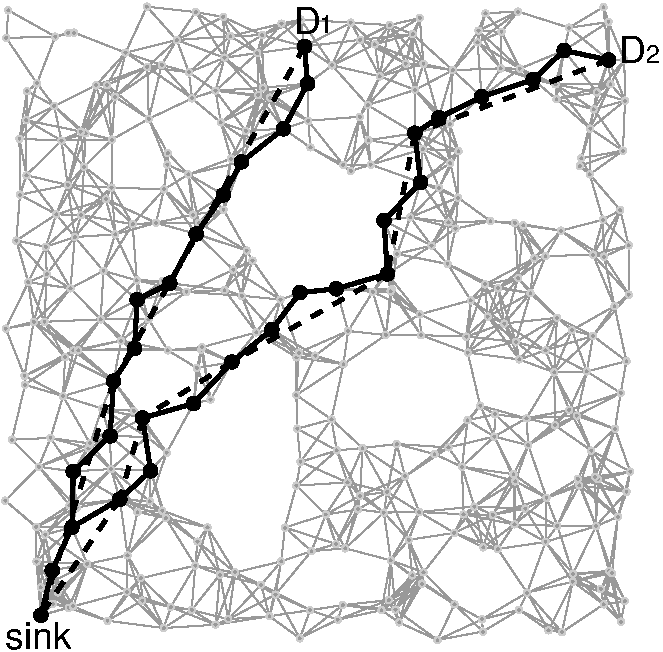
\includegraphics[width=0.55\textwidth]{fig511}
\caption{网络均匀性对PathZip-G的压缩率的影响}
\label{fig:511}
\end{figure}

5. 网络部署均匀性

下面评估网络部署的均匀性对PathZip-G的压缩率的影响。

我们利用具有不同扰动系数的扰动网格模型生成具有不同均匀性的网络,分别从每个网络中选择1000个节点对,并计算PathZip-G在不同网络中的平均压缩率。图\ref{fig:510f}给出了实验结果,其中$x$轴表示扰动网格模型的扰动系数,$y$轴表示不同网络中压缩率的平均值。实验结果显示,压缩率随着网络均匀性的增加而稍有波动,但没有表现出明显的趋势。可见,PathZip-G对网络部署的均匀性同样具有良好的鲁棒性。

6. 网络空洞的影响

最后评估网络空洞对PathZip-G压缩率的影响。首先从直观上分析,当数据包通过的网络区域中包含较多形状复杂的空洞时,其传输路径也将呈现出频繁的变化,因此对应的虚拟路径将可能包含更多的节点,从而导致压缩率下降。下面通过仿真实验对这一分析结果进行验证。

在图\ref{fig:511}所示的网络中,黑实线分别表示了从两个节点$D_1$和$D_2$到汇聚节点的传输路径,虚线表示在相同的误差上限设置下(节点通讯半径的1/2),两条路径分别对应的虚拟路径。可见,节点$D_1$的路径通过的区域较均匀,因此其对应的虚拟路径的压缩率更高(具体为5);而节点$D_2$由于其路径通过的网络区域形状较复杂,其对应的虚拟路径的压缩率较低(具体为2.86)。

\section{本章小结}
路由路径记录是无线传感器网络拓扑压缩技术的重要研究内容,对于改善网络状态的可见性以及提供细粒度的网络管理功能具有重要的作用。目前的相关研均究无法获得网络中每个数据包的完整路径信息。本章首次正式地提出和系统地研究无线传感器网络的路由路径记录问题,设计了一种轻量级的,在实际的大规模网络中可用的路由路径记录方法,称为PathZip。本章设计了一种基于哈希的路径压缩和恢复方法,能够有效地追踪和记录网络中的每个数据包的完整的路由路径,同时保证传感器节点的计算开销和存储开销均较低。另外,本章还设计了分别基于拓扑和基于几何的技术,通过开发路径之间的拓扑相关性和集合相关性来有效地降低算法的开销。本章通过理论分析和大量的仿真实验验证了PathZip方法的有效性和性能,结果显示PathZip能够在较低的计算和存储开销下,实时地记录网络中每个数据包的完整和精确的传输路径。
